\documentclass[a4paper,11pt, twoside]{article}
%\documentclass[a4paper,11pt]{scrartcl}
\usepackage[a4paper,top=3cm,bottom=3.5cm,left=2.5cm,right=2.5cm]{geometry}
\usepackage{graphicx}
\usepackage[utf8x]{inputenc}
\usepackage[italian]{babel}
\usepackage{fancyhdr}
\usepackage{amssymb}
\usepackage{makeidx}
\usepackage{eurosym}

\usepackage{amsthm}

\theoremstyle{definition}
\newtheorem{defn}{Definizione}[section]



\title{Appunti di Basi di Dati 2}
\author{Matteo Gianello}
\date{\today}

\pdfinfo{%
  /Title    (Appunti di Basi di Dati 2)
  /Author   (Matteo Gianello)
  /Creator  (Matteo Gianello)
  /Producer ()
  /Subject  ()
  /Keywords (Basi Dati 2 Campi IngInf Polimi)
}

\begin{document}
\pagestyle{empty}
\thispagestyle{empty}
\maketitle
\newpage

\thispagestyle{plain}
\tableofcontents
\newpage

\pagestyle{plain}
\label{capitolo1}
\section{Gestione delle transizioni}
\subsection{Le transizioni}
Una transizione � un unit� elementare di lavoro svolta da un applicaazione; mentre un applicazione pu� essere formata da una serie di transizioni.\\
Per meglio specificare una transizione � formata da una sequenza di operazioni racchiusa da una coppia di istruzioni che ne specificano l'inizio e la fine.
In  particolare esistono 2 tipi di operazioni di fine transizione, il \emph{commit work} e il \emph{rollback work}; che richiedono rispettivamente una conclusione positiva e negativa della transizione.\\
Una conclusione positiva della transizione implica una aggiornamento della base di dati; nel caso invece di un rollback i cambiamenti non vengono apportati alla base di dati.\\
In caso di operazioni articolate � necessario introdurre il concetto di \emph{transizione ben formata} che prevede un inizio \textsf{start transiction} e una fine ideale \textsf{end transiction} nel corso della transizione viene eseguito uno solo dei comandi \textsf{commit} o \textsf{rollback} e in cui non avvengono operazioni sulla base di dati dopo l'esecuzzioni di uno di questi due comandi.
\subsubsection{Propriet� "acide" delle transizioni}
Le transizioni, in quanto svolte in ambienti piuttosto critici, devono goderedi alcune propriet� particolari dette \emph{acide}: atomicit�, consistenza, isolamento e persistenza.
\begin{description}
    \item[Atomicit�] rappresenta il fatto che una transizione � un'unit� \emph{indivisibile} di esecuzione; o viene eseguita e resa visibile l'intera transizione oppure non deve esserci nessun effetto sulla base di dati.
Questo significa che nel caso di un guasto durante la transizione il sistema deve riportare la base di dati nel suo stato iniziale (\emph{undo}) mentre dopo l'essecuzione di un commit il sistema deve rieseguire le operazioni per applicare le modifiche (\emph{redo)}. Nel caso invece di un rollback il sistema uccide la transizione, questa operazione � detta di \emph{abort}.\\
	\item[Consistenza] richiede che tutte le transizioni non violino i vincoli di integrità definiti sulla base di dati. La verifica di questi vincoli � di tipo immediato gestendo nel programma le condizioni anomale e rimuovendone gli effetti.\\
	\item[Isolamento] forse la pi� importante delle propriet� acide richiede che l'esecuzione di una transizione sia indipendente dalla contemporanea esecuzione di altre transizioni; ovvero si richiede che il risultato di esecuzioni concorrenti sia uguale al risultato delle singole transizioni eseguite da sole.\\
	\item[Persistenza] questa propriet� richiede che l'effetto di una transizione che ha eseguito correttamente il commit non venga pi� perso.
\end{description}

\subsection{Controllo di concorrenza}
Un DBMS deve servire diverse applicazioni contemporaneamente e rispondere a richieste di diversi utenti. Per questo � necessario che le transizioni in un DBMS vengano eseguite concorrentemente.
\subsubsection{Anomalie delle transizioni concorrenti}
L'esecuzione concorrente di varie transizioni pu� portare ad alcuni problemi di correttezza o anomalie.
\paragraph{Perdita di aggiornamento} 
$$r_1(x),r_2(x),w_2(x),c_2,w_1(x),c_1$$
In questo caso come si nota non si registrano gli effetti della transizione $t_2$ in quanto mascherata dalla prima transizione.
\paragraph{Lettura sporca}
$$r_1(x),w_1(x),r_2(x),a_1,c_2$$
In questo caso la transizione $t_2$ va a leggere un dato che in realt� � errato in quanto la prima transizione dopo aver eseguito le operazioni esegue un \emph{abort}
\paragraph{Lettura inconsistente}
$$r_1(x),r_2(x),w_2(x),c_2,r_1(x)$$
In questo caso la transizione $t_1$ legge due volte il dato \emph{x} che per� � stato modificato da $t_2$; questo comportamento non � tollerato in quanto si vuole che una transizione che accede due volte alla base di dati trovi esattamente lo stesso valore.
\paragraph{Aggiornamento fantasma} Prendiamo in considerazioni tre dati \emph{x, y, z} che soddisfano un vincolo di integrit� del tipo $x+y+z=1000$
$$r_1(x),r_2(y),r_1(y),y-100,r_2(z),z+100,w_2(y),w_2(z),c_2,r_1(z),c_1$$
In questo caso la transizione $t_1$ non rispetta pi� i vincoli di integrit� in quanto legge il valore di \emph{y} prima dell'update e quello di \emph{z} dopo.
\paragraph{Inserimento fantasma}
\subsubsection{Teoria del controllo di concorrenza}
Prima di definire la precisamente i problemi posti dalla concorrenza diamo alcune definizioni un po pi� rigorose.\\
Definiamo una transizione come una sequenza di operazioni di lettura o scrittura ad esempio:
$$t_1: \ r_1(x),r_1(y),w_1(x),w_1(y)$$
Uno \emph{schedule} � una sequenza di operazioni di ingresso/uscita presentate da trasinzioni concorrenti:
$$S_1: \ r_1(x),r_2(z)w_1(x),w_2(z) \dots$$
Le transizioni compaiono nello schedule seguendo l'ordine temporale con cui sono eseguite sulla base di dati.\\
La funzione di un controllo di concorrenza � quella di accettare alcuni schedule e rifiutarne degli altri in modo da evitare che si verifichino le anomalie presentate in precedenza. 
Il modulo che gestisce il controllo di concorrenza � perci� chiamato \emph{scheduler}.\\
Innanzitutto ci occuperemo di schedule \emph{commit-proiezione} ovvero schedule nei quali l'esito delle trransizioni � noto e che contengono cos� solo le transizioni che producono un commit.\\
Definiamo \emph{seriale} uno schedule in cui le azioni di ciascuna transizione compaiono in sequenza senza essere frammentate da istruzioni di altre transizioni.
$$S_2: \ r_0(x),r_0(y)w_0(x),r_1(y)r_1(x)w_1(y)r_2(x)r_2(y)r_2(z)w_2(z)$$

L'esecuzione della commit-proiezione di uno schedule $S_i$ � corretta quando produce un risultato equivalente ad un qualunque schedule seriale $S_j$ con le stesse transizioni. In tal caso lo schedule $S_i$ si dice \emph{serializzabile}
\paragraph{View-equivalenza} Prima di definere che cos'� la view-equivalenza definiamo alcune relazioni che legano coppie di operazioni di lettura e scrittura. Una lettura $r_i(x)$ \emph{legge da} una scrittura $w_j(x)$ quando $w_j(x)$ precede $r_i(x)$ e non vi � alcun $w_k(x)$ compresa tra le due.
Una scrittura $w_i(x)$ viene detta \emph{scrittura finale} se � l'ultima scrittura sull'oggetto \emph{x}.\\
Due schedule vengono detti \emph{view-equivalenti} ($S_i \approx_V S_j$) se possiedono le stesse relazioni \emph{legge-da} e le stesse \emph{scritture fianli}.
Uno schedule � detto \emph{view-serializzabile} se esiste uno schedule seriale \emph{view-equivalente} ad esso.\\
Determinare la view-equivalenza di uno schedule � un problema con complessit� lineare; ma determinare se uno schedule � view-equivalente a un qualisiasi schedule seriale � un problema NP-difficile. Questo risultato fa si che la view-equivalenza non sia utilizzabile per caratterizzare la serializzabilit� di uno schedule.
\paragraph{Conflict-equivalenza} Date due azioni $a_i$ e $a_j$ con $i \neq j$ si dice che $a_i$ � in \emph{conflitto} con $a_j$ se esse operano sullo stesso oggetto e almeno una di essa � una scrittura.
Possono perci� esistere conflitti lettura-scrittura (\emph{wr,rw}) oppure conflitti scrittura scrittura (\emph{ww}).\\
Si dice che lo schedule $S_i$ � \emph{conflic-equivalente} allo schedule $S_j$ ($S_i \approx_C S_j$) se i due schedule presentano le stesse operazioni e ogni cocoppia di operazioni in conflitto � nello stesso ordine nei due schedule. Uno scschedule � \emph{conflict-serializzabile} se esiste uno schedule seriale a esso conflict-equivalente.\\
LaLa classe degli schedule CSR � strettamente inclusa in quelli VSR esistono cio�, schedule che appartengono alla classe VSR ma non CSR.\\
Il calcolo della conflict-serializzabilità � semplice, basta calcolare il \emph{grafo dei conflitti} costruito facendo corrispondere un nodo a ogni transizione e un arco orientato da $t_i$ a $t_j$ se esiste almeno un conflitto tra una azione $a_i$ e un'azione $a_j$. A questo punto si pu� dimostrare che uno schedule e CSR se e solo se il suo grafo dei conflitti � aciclico.\\
Nonostante la fattibilit� del metodo CSR la sua implementazione in ambito commerciale risulta ancora troppo onerosa e inaccettabile.
\paragraph{Locking a due fasi} Il meccanismo pi� diffuso per il controllo di concorrenza si basa sul \emph{locking}, un meccanismo molto semplice che impone che tutte le operazioni di lettura e scrittura siano protette attraverso l'esecuzione di opportune primitive \textsf{r\_lock, w\_lock, unlock}; lo scheduler (o in questo caso anche \emph{lock manager}) riceve una sequenza di richieste di esecuzione di queste primitive e ne verifica la correttezza semplicemente \emph{ispezionando} la struttura dati.\\
Esistono alcuni vincoli da rispettare: 
\begin{enumerate}
\item Ogni operazioni di lettura deve essere preceduta da un \textsf{r\textunderscore lock} e seguita da un \textsf{unlock}; in questo caso il lock si dice \emph{condiviso} perch� su un dato possono essere attivivi pi� lock di questo tipo.
\item Ogni operazione di scrittura deve essere preceduta da un \textsf{w\_lock} e seguita da \textsf{unlock} in questo caso il lock si dice \emph{esclusivo} in quanto non pu� coesistere con altri tipi di lock.
\end{enumerate}
Queste regole non sono strette perci� una transizione pu� richiedere un lock molto prima di effettuare tale operazione. Oppure potrebbe chiedere un \emph{lock upgrade} in caso debba compiere prima un'operazione di lettura e poi una di scrittura passando da un r\_lock a un w\_lock.\\
I meccanismi di lock garantiscono che le transizioni che accedono alla base di dati operino in mutua esclusione; ma per avere la garanzia che queste seguano uno schedule serializzabile � necessario porre una restrizione sull'ordinamento delle richieste di lock, questo principio prende il nome di \emph{locking a due fasi} (2PL).\\
\begin{center}
\emph{Una transizione, dopo aver rilasciato un lock, non pu� acquisirne altri.}\\
\end{center}
Utilizzzando questo principio si possono distinguere nell'esecuzione di una transizione due diverse fasi: una prima fase detta (\emph{crescente}) nella quale si acquisiscono i lock alle risorse alle quali bisogna accedere; una seconda fase (\emph{calante}) nella quale i lock acquisiti vengono rilasciati.\\
La classe degli schedule 2PL � strettamente contenuta in quella CSR.\\
Fino ad ora abbiamo lavorato immaginando che i nostri schedule non producessero mai un abort (commit-proiezione); ora possiamo estendere il meccanismo di locking a due fasi per fare in modo che anche quegli schedule con anomalie dovute agli abort delle transizioni (lettura sporca). Per rimuovere quindi la commit-proiezione restringiamo il protocollo 2PL, facendolo cos� diventare il cos� detto \emph{2PL strict}.\\
\begin{center}
\emph{I locking di una transizione possono essere rilasciati solo dopo aver correttamente effettuato le operazioni di commit/abort.}\\
\end{center}
\paragraph{Controllo di concorrenza basato su timestamp} Questo meccanismo, pi� semplice ma meno efficace del locking a due fasi, utilizza i \emph{timestamp} cio� identificatori associati ad ogni evento temporale che definiscono un ordinamento totale sugli eventi. Il controllo di concorrenza avviene nel seguente modo:
\begin{itemize}
\item a ogni transizione si associa un timestamp che presenta il momento di inizio della transizione;
\item si accetta uno schedule solo se esso riflette l'ordinamento seriale delle transizioni in base al valore del timestamp di ciascuna transizione.
\end{itemize}
A ogni oggetto $x$ vengono associati due indicatori, WTM(x) e RTM(x) che indicano rispettivamente il timestamp pi� alto delle transizioni che hanno scritto e letto il dato $x$. Allo scheduler arrivano le richieste di accesso agli oggetti e queste vengono accettate o rifiutate secondo le seguenti regole:
\begin{itemize}
\item $r_t(x)$: se $t < WTM(X)$ la transizione viene uccisa, altrimenti la richiesta viene accettata e l'idicatore RTM(x) viene aggiornato con il massimo tra RTM(x) e $t$.
\item $w_t(x)$: se $t < WTM(x) o t < RTM(x)$ la transizione viene uccisaaltrimenti la richiesta viene accettata e il valore di WTM(x) viene posto pari a $t$.
\end{itemize}
Il metodo TS comporta l'uccisione di un gran numero di transizioni ed � corretto solo se si bufferizzano le scritture e le si copiano sulla base di dati solo a commit avvenuto.\\
Un metodo alternativo e pi� efficace consiste nel creare una copia ogni qualvolta una scrittura viene accettata; in questo caso le letture non vengono mai rifiutate ma vanno dirette alla copia del dato con il timestamp adeguato, mentre le scritture vengono accettate solo se il loro timestamp � maggiore di RTM(x) ed in tal caso si crea una nuova copia del dato.\\
\subsubsection{Meccanismi per la gestione dei lock}
Come abbiamo visto nel precedente paragrafo il lock � il meccanismo pi� diffuso per quanto riguarda i DB commerciali. Fino ad ora per� abbiamo supposto che il lock bloccasse tutte le risorse.\\
In realt� esiste un meccanismo chiamato \emph{lock gerarchico} che permette una granularit� pi� fine sul lock delle risorse. Esso mette a disposizione un maggior numero di primitive:
\begin{itemize}
\item XL: lock esclusivo, corrisponde al write-lock
\item SL: lock condiviso, corrisponde al read-lock
\item ISL: intenzione di lock condiviso, esprime l'intenzione di bloccare in modo condiviso uno dei sottonodi del nodo a cui si applica.
\item IXL: intenzione di lock esclusivo, esprime la volont� di bloccare in modo esclusivo uno dei nodi figli.
\item SIXL: lock condiviso con intenzione di lock esclusivo, blocca il nodo corrente in modo condiviso ma esprime l'intenzione di bloccare in modo esclusivo uno dei sottonodi.
\end{itemize}
\subsubsection{Blocco critico}
Il blocco critico o \emph{deadlock} � una situazione nella quale due transizioni rimangono in attesa di acquisire un lock che richiederebbe la terminazione di una delle due transizioni per essere concesso.
Esistono diversi meccanismi per� per evitare che ci� accada:
\begin{enumerate}
\item timeout
\item prevenzione
\item rilevamento
\end{enumerate}
\paragraph{Timeout} La tecnica pi� semplice che implica che le transizioni rimangano in attesa di una risorsa per un tempo prefissato, se passa questo tempo e la risorsa non � stata concessa allora la richiesta di lock viene negata e la transizione abortita.
\paragraph{Prevenzione dei blocchi critici} Vi sono diverse tecniche per prevenire i deadlock; una � quella di richiedere i lock su tutte le risorse in una volta sola. Un'altro metodo si basa sul controllo dei timestamp e di concedere l'attesa di una risorsa solo se chi l'ha bloccata ha un timestamp maggiore.
Questi meccanismi tendono per� a non essere molto efficenti e perci� non vengono spesso implementato nei DBMS commericali.
\paragraph{Rilevamento dei blocchi critici} Pi� comune � l'uso del rilevamento dei blocchi critici. Questo meccanismo viene implementato nel seguente modo; il gestore di concorrenza concede i lock alle varie transizioni salvando in una tabella l'identificativo della transizione e le risorse da essa bloccate.\\
Periodicamente il controllore di concorrenza analizza la tabella dei lock e crea il grafico dei conflitti; una volta creato il grafico controlla se in esso sono presenti dei cicli.\\
Questo meccanismo soprattutto quando eseguito periodicamente risulta molto efficente ed �  usato da molti vendor.

\subsection{Controllo di affidabilit�}
Il controllo di affidabilit� garantisce \emph{l'atomicit�} e la \emph{persistenza} delle transizioni; ovvero esso permette che le transizioni non vengano lasciate incomplete e che gli effetti di ciascuna transizione conclusa siano mantenuti in modo permanente.\\
Il controllo di affidabilit� � svolto dal rispettivo controllore e viene implementato attraverso il \emph{log} sul quale vengono memorizzate tutte le azioni svolte dal DBMS (\emph{DataBase Management System}).
\subsubsection{Architettura del controllore di affidabilit�}
Il controllore di affidabilita� ha il compito di realizzare i comandi \textsf{start transiction, comit, rollback} e di realizzare le operazioni di ripristino dopo i malfunzionamenti dette \emph{ripresa a caldo} e \emph{ripresa a freddo} ed infine predisponei dati necessari per eseguire meccanismi di ripristino dai guasti in particolare azioni di \emph{checkpoint} e di \emph{dump}.
\subsubsection{Organizzazione del log}
Il \emph{log} � un file sequenziale in sono contenute informazioni ridondante che permettono di ricostruire il contenuto della base di dati a seguito di guasti. Vengono registrate le azioni svolte dalle varie transizioni nell'ordine temporale delle stesse.\\
I record del log sono di due tipi:
\begin{itemize}
\item di transizione
\item di sistema
\end{itemize}
I record di transizione registrano le attivit� svolte da ciascuna transizione nell'ordine in cui vengono effettuate; ovvero vengono inseriti i record di \textsf{begin} i vari record relativi alle azioni eseguite (\textsf{insert, delete, update})e uno dei due record \textsf{commit} oppure \textsf{abort}.\\
I record nei log vengono cos� indicati:
\begin{itemize}
\item I record di \textsf{begin, commit e abort} contengono oltre all'ndicazione del tipo di operazione anche un identificativo della transizione che viene eseguita (\emph{B($T_i$),C($T_i$),A($T_i$)})
\item Il record \textsf{update} oltre all'identificativo della transizione contiene l'identificativo dell'oggetto sul quale si effettua l'operazione \emph{O} e lo stato prima e dopo la modifica indicati rispettivamente da \emph{BS (before state)} e \emph{BS (After state)}.
\item I record \textsf{insert} e \textsf{delete} sono simili all'update solo che mancano dei campi rispettivamente di BS e AS.
\end{itemize}
L'utilizzo di questi record permette di disfare e rifare le azioni in caso di guasto; le azioni che svolgono questa funzione sono:
\begin{itemize}
\item Primitiva di \emph{Undo} che disfa le azioni su un oggetto O ricopiando in tale oggetto il valore BS mentre per l'insert si cancella semplicemente l'oggeto.
\item Primitiva di \emph{Redo} che riesegue le operazioni su un oggetto O ricopiando il valore AS e nel caso di delete ricreando l'oggetto cancellato.
\end{itemize}
Per quanto riguarda i due record di sistema abbiamo il \emph{checkpoint} e il \emph{dump}.
Il checkpoint � un operazione che viene svolta periodicamente con l'obiettivo di registrare quali transizioni sono attive. Una versione semplitificata ed intuitiva delle operazioni che vengono svolte � la seguente:
\begin{enumerate}
\item Si sospende l'accettazione di operazioni di scrittura, commit o abort da parte di qualunque transizione.
\item Si trasferiscono in memoria di massa tutte le pagine del buffer.
\item Si scrive in modo sincrono nel log il record di checkpoint specificando le transizioni attive.
\item Si riprende l'accettazione delle operazioni sospese.
\end{enumerate}

Un \emph{dump}, invece, � una copia completa della base di dati effettuata in muta esclusione con tutte le transizioni quando il sistema non � operativo.
Dopo l'operazione di dump viene scritto il relativo record sul log.
\subsubsection{Esecuzione delle transizioni e scrittura sul log}
Per ripristinare la base di dati in caso di guasti � necessario che durante il normale svolgimento delle transizioni il controllore di affidabilit� garantisca due regole nella scrittura dl log:
\begin{itemize}
\item La regola \emph{WAL (Write Ahead Log)} impone che la parte \emph{before state} dei record di un log sia scritta sul log prima di effetuare la corrispondente operazione sulla base di dati. 
\item La regola di \emph{Commit-Precedenza} impone che la parte \emph{after state} dei record venga scritta nel lo prima di effettuare il commit.
\end{itemize}
La transizione infine scrive in modo sincrono il record di commit; cos� facendo un eventuale guasto prima di questa operazione comporta l'\emph{Undo} di tale operazionem mentre un guasto dopo il record di commit implica l'esecuzione in caso di guasto della primitiva \emph{Redo}.
\subsubsection{Gestione dei guasti}
Dal punto di vista di un DBMS i guasti si suddivido in due classi:
\begin{itemize}
\item \emph{Guasti di sistema:} sono guasti introdotti da problemi software oppure dovuti a malfunzionamenti dei dispositivi che portano il sistema in uno stato inconsistente. Questi portano ad una perdita dei dati in memoria centrale ma la memoria di massa rimane consistente.
\item \emph{Guaasti del dispositivo:} sono guasti relativi ai dispositivi di memorizzazione di massa; in questo caso si ha una perdita totale della base di dati ma non del log.
\end{itemize}
Il modello ideale nel quale noi ci poniamo � detto \emph{fail-stop} ovvero quando il sistema individua un guasto esso arresta tutte le transizioni e ripristina il corretto funzionamento del sistema. Nel caso di guasto di sistema si effetua una \emph{ripresa a caldo} mentre nel caso di guasto dispositivo si effettua una \emph{ripresa a freddo}
\paragraph{Ripresa a caldo} La ripresa a caldo si articola nelle seguenti fasi:
\begin{enumerate}
\item Si accede all'ultimo record del log e si ripercorre all'indietro fino all'ultimo e pi� recente record di checkpoint.
\item Si decidonmo le transizioni da rifare o disfare; si costruiscono due insiemi UNDO e REDO e si inizializza l'insieme di UNDO con le transizioni attive al momento del checkpoint. Inoltre si aggiungono a tale insieme tutte le transizioni che presentano nel log un record di \emph{begin} mentre si spostano nell'insieme REDO quelle che presentano il record di commit.
\item Si ripercorre nuovamente all'indietro il log disfacendo quelle dell'insieme UNDO.
\item Infine si rifanno le transizioni presenti nell'insieme REDO.
\end{enumerate}
\paragraph{Ripresa a freddo} La ripresa a freddo consiste in tre fasi:
\begin{enumerate}
\item Nella prima fase si accede al dump e si ricopia selettivamente la parte deteriorata della base di dati e si ritrova nel log il pi� recente record di \emph{dump}.
\item Si ripercorre in avanti il log rieseguengo tutte le operazioni descritte in modo da riportarsi alla situazione precedente al guasto.
\item Si esegue una ripresa a caldo.
\end{enumerate}

\label{capitolo2}
\section{Basi di dati distribuite}
Fino ad ora abbiamo studiato i meccanismi delle transizioni trascurando i componenti fisici sui quali la base di dati risiede e quindi immaginando che essa sia unica.\\
In quai la totalit� dei casi invece le basi di dati sono \emph{distribuite} ovvero risiedono su diverse macchine collegate tra loro da una rete.\\
L'architettura distribuita pi� semplice � quella \emph{client-server} dove una serie di client gestiscono l'interazione con l'utente e sono connesse a una serie di server.\\
I problemi iniziano per� nel caso in cui due o pi� server siano collegati tra loro e debbano effettuare delle transizioni distribuite. Le maggiori difficolt� in questo caso si hanno nel garantire le propriet� "acide" delle transizioni. Per gestire tali casi studieremo il protocollo pi� diffuso chiamato protocollo di \emph{commit a due fasi}.
Dalla nascita del contesto distribuito le basi di dati hanno iniziato a distinguersi in due categorie:
\begin{itemize}
\item La prima finalizzata alla gestione dei dati in linea (real-time) denominata \emph{On-Line Transiction Processing, OLTP} nella quale le architetture sono dimensionate per gestire centinaia o migliaia di transizioni al secondo.
\item La seconda categoria � finalizzata all'analisi dei dati o \emph{On-Line Analytical Processing, OLAP} realizzate attraverso le \emph{data warehouse}.
\end{itemize}
\subsection{Architettura client-server}
Il paradigma client-server prevede due attori i processi \emph{client} che richiedono i servizi e i \emph{server} che forniscono i servizi. I client hanno lo scopo di interfacciarsi con l'utente e generano in modo autonomo "poche" richieste ad un server, perci� essi sono definiti processi attivi; i server invece rispondono a "molte" richieste da parte di diversi client perci� sono definiti processi \emph{reattivi}.\\
I server sono molto spesso \emph{multi-thread} ovvero possono gestire pi� di una transizione per volta. Ciascuna unit� che gestisce una transizione � chiamata \emph{thread}; le richieste in arrivo al server e i risultati vengono immagazzinati in code fino alla loro gestione; queste code sono rispettivamente la \emph{coda di ingresso} e la \emph{coda di uscita}. Esse sono gestite o dal server stesso o da un altro processo detto \emph{dispacher}.
\subsection{Basi di dati distribuite}
\subsubsection{Applicazioni delle basi di dati distribuite}
La decisione di avere una basi delle basi di dati distribuite � nata in quanto nelle imprese si ha una divisione delle informazioni nei diversi settori dell'azienda. Inoltre i sistemi distribuiti hanno prevarso su quelli centralizzati in quanto pi� flessibili, pi� resistenti ai guasti e meno soggetti a degrado delle prestazioni.\\
Una prima classificazione delle basi di dati distribuite considera il tipo di DBMS utilizzato, infatti se i diversi server utilizzano lo stesso DBMS si parla di una base di dati \emph{omogenea} altrimenti essa � \emph{eterogenea}.
Inoltre una base di dati pu� utilizzare una \emph{rete locale LAN} oppura una \emph{rete geografica WAN}
\subsubsection{Autonomia locale e cooperazione}
Una base di dati distribuita garantisce comunque ai programmi applicativi esattamente lo stesso tipo di interazioni che si avrebbe con un sistema centralizzato. Ma un sistema distribuito non ha lo scopo di massimizzare l'interazione tra i server ma al contrario un progetto accurato di una base di dati distribuita dovrebbe garantire che la maggior parte delle applicazioni si svolga in modo autonomo su di un solo server in modo da non dover aumentare il tempo di esecuzione a causa della latenza dovuta all'interazione.
\subsubsection{Frammentazione e allocazione dei dati}
La frammentazione dei dati consente di organizzare gli stessi in modo tale da garantire una distribuzione efficente e ben organizzata; ma per essere tale questa tecnica deve essere pianificata a piori.\\
Possiamo avere due tipi di frammentazione \emph{orizzontale} o \emph{verticale}:
\begin{itemize}
\item Nella \emph{frammentazione orizzontale} i frammenti $R_i$ sono insiemi di tuple con lo stesso schema di relazione di $R$; pu� essere interpretato come il risultato di una selezione applicata ad $R$.
Esempio divido i dati dei dipendenti in due, quelli che hanno uno stipendio minore di 1000\EUR e quelli con stipendio maggiore.
\item Nella  \emph{frammentazione verticale} i frammenti $R_i$ hanno uno schema ottenuto come sottoinsieme dello schema di $R$.
\end{itemize}
La frammentazione � corretta se e solo se sono rispettate le seguenti propriet�:
\begin{itemize}
\item \emph{completezza:} ogni dato della relazione R deve essere presente in qualche suo frammento. 
\item  \emph{ricostruibilit�:} la relazione deve essere interamente ricostruibile a partire dai suoi frammenti.
\end{itemize}
Lo \emph{schema di allocazione} contiene il mapping dei frammenti sui server che lo memorizzano consentendo il passaggio da una descrizione logica a una fisica.
Tale mapping pu� essere:
\begin{itemize}
\item \emph{non ridondante} se un frammento � allocato esattamente su un server.
\item \emph{ridondante} quando qualche frammento o relazine viene collocato su pi� server.
\end{itemize}
\subsubsection{Livelli di trasparenza}
Esistono diversi livelli di trasparenza che permettono di scrivere applicazioni a diverso livello. I principali tipi di trasparenza sono tre: trasparenza di frammentazione, di allocazione, e di linguaggio; vi � in oltre la possibilit� di una totale assenza di trasparenza.
\begin{itemize}
\item \emph{Trasparenza di frammentazione} a questo livello il programmatore non si preoccupa della framentazione della base di dati ma a questo livello viene trattata come se la base di dati fosse situata su un unica macchina.
\item \emph{Trasparenza di allocazione} In questo caso il programmatore conosce il grado di frammentazione della base di dati ma non si preoccupa di dove essa sia situata .
\item \emph{Trasparenza di linguaggio} Il programmatore conosce tutto sulla framentazione e l'allocazione della base di dati e quindi la singola interrogazione deve essere mirata al giusto frammento. L'unica cosa che viene ancora ignorata � il linguaggio di intterrogazione che � unico per tutti i frammenti e allocazioni; esso � indipendente dal DBMS.

\end{itemize}
\subsubsection{Classificazione delle transizioni}
Un client collegato a un server con un certo DBMS pu� inviare ad esso transizioni \emph{locali} ovvero destinate a dati presenti nel server oppure transizioni \emph{non locali} destinate a dati situati su altri DBMS; queste transizioni possono essere distinte in categorie:
\begin{description}
\item [richieste remote] sono transizioni di sola lettura ed indirizzate ad un solo DBMS remoto
\item [transizioni remote] sono transizioni costituite da un numero qualsiasi di comandi SQL e destinate a un solo DBMS.
\item [transizioni distribuite] sono transizioni rivolte a un generico numero di DBMS ma in cui ogni comando SQL � rivolto a uno specifico DBMS
\item [richieste distribuite] sono tranzizioni arbitrarie costituite da un numero arbitrario di operazioni SQL nelle quali ogni query pu� fare riferimento a dati distribuiti su diversi DBMS.
\end{description}
\subsection{Tecnologia delle basi di dati distribuite}
La distribuzione dei dati non influisce sulle propriet� acide di consistenza e persistenza:
\begin{itemize}
\item \emph{consistenza} delle transizioni non dipende dalla distribuzione dei dati, i vincoli di integrit� esprimono solo propriet� locali dei DBMS; questo � dovuto soprattutto per la mancanza di meccanismi che permettano di far riferimento a dati distribuiti.
\item \emph{persistenza} non � un problema che dipende dalla distribuzione dei datiin quanto ogni DBMS garantisce la persistenza attraverso meccanismi di backup e dump locali.
\end{itemize}
\subsubsection{Ottimizzazione di interrogazioni distribuite}
L'ottimizzazione delle interrogazioni � richiesta soltanto quando trattiamo le richieste distribuite in cui cio� dati distribuiti sono coinvolti nella stessa interrogazione.\\
Il DBMS al quale viene sottoposta l'intterrogazione si occupa della cosiddetta \emph{ottimizzazione globale}, ovvero della decomposizione in sotto-interrogazioni rivolte ad uno specifico DBMS.\\
Le operazioni che vengono svolte sono: scegliere l'ordine delle operazioni e il loro metodo di esecuzione, si definisce la strategia di esecuzione nel caso in cui gli operandi siano allocati su nodi distinti definendo anche una strategia per la trasmissione dei risultati, nel caso di dati ridondanti � necessario decidere a quale copia di dati accedere. Per aiutare in tale decisione si associa a ogni nodo foglia un costo che prevede il contributo di tre componenti:
$$C_{total} = C_{I/O} \times n_{I/O} + C_{cpu} \times n_{cpu} + C_{tr} \times n_{tr}$$
dove $n_{tr}$ e $C_{tr}$ misurano rispettivamente la quantit� di dati trasmessi in rete e il loro costo unitario.
\subsubsection{Controllo di concorrenza}
In un sistema distribuite una transizione $t_i$ pu� essere formata da varie sotto-transizioni $t_{ij}$ dove il secondo indice indica il nodo sul quale la sotto transizione viene eseguita. Inoltre possiamo dimostrare come la serializzabilit� locale non sia condizione necessaria e sufficiente a garantire la serializzabilit� di due transizioni.
\paragraph{Serializzabilit� globale} La \emph{serializzabilit� globale} di due transizioni distribuite richiede l'esistenza di un \emph{unico schedule seriale S} che coinvolga tutte le transizioni del sistema e che sia comune a tutti gli schedule locali $S_j$. Questo significa che la proiezione $S[j]$ di S contenente le sole azioni che S svolge sul nodo j sia uguale allo schedule locale $S_j$.\\
Questo propriet� risulta immediata nel caso di uso di locking a due fasi o di timestamp.
\begin{itemize}
\item Se ciascuno scheduler su ogni nodo della base di dati distribuita usa il metodo 2PL strict e quindi svolge l'azione di commit in modo atomico, cio� quando tutte le risorse sui vari nodi sono bloccate gli schedule risultanti sono globalmente serializzabili.
\item Se un insieme di sotto-transizioni distribuite acquisisce un unico timestamp e usa tale timestamp nelle richieste a tutti gli scheduler gli schedule risultanti sono globalmente serializzabili.
\end{itemize}
\paragraph{Metodo di Lamport per assegnare i timestamp} Per garantire il buon funzionamento del metodo di concorrenza basato su timestamp � necessario che la transizione distribuita riceva il timestamp relativo all'istante in cui si sincronizza con le altre transizioni; per questo si usa il \emph{metodo di Lamport} che riflette le relazioni di precedenza in un sistema distribuito.\\
Un timestamp � caratterizzato da due gruppi di cifre il meno significativo indica il nodo mentre il pi� significativo il numero di eventi che accadono su ciascun nodo ricavato da un contatore locale che viene incrementato ad ogni evento.\\
Inoltre i timestamp si sincronizzano ogni qualvolta che due nodi comunicano aggiornando in quanto il timestamp dell'evento di ricezione deve avere un timestamp successivo a quello di invio.
\paragraph{Rilevazione distribuita dei deadlock} Quando i deadlock coinvolgono transizioni distribuite la loro rilevazione � pi� complessa  in quanto i deadlock possono essere dovuti a situazioni di attesa circolare che si verificano su due o pi� nodi. La soluzione pi� semplice e pi� diffusa � sicuramente quella dell'uso dei timeout.\\
Esiste per� un altro algoritmo abbastanza efficente che permette la rilevazione dei deadlock distribuiti. Questo � un algoritmo distribuito che viene attivato periodicamente dai vari DBMS. Quando � attivo esso analizza la situazione di attesa sul suo nodo e comunica con le altre istanze la sua \emph{sequenza di attesa}; per evitare che lo stesso deadlock venga rilevato da pi� transizioni il messaggio viene propagato solo al DBMS ove � attiva la sotto-transizione attesa e se ad esempio il nodo ricevente ha un id maggiore di quello che invia.\\
L'algoritmo opera come segue:
\begin{enumerate}
\item I messaggi provenienti da altri DBMS vengono letti e l'informazione viene composta in un grafo di attesa locale e le transizioni remote in attesa vengono aggiunte al grafo locale.
\item Viene svolta una ricerca locale di deadlock e situazioni di stallo vengono risolte da degli abort.
\item Vengono computate le sequenze di attesa remote e inviate ai DBMS remoti in avanti.
\end{enumerate}
\subsubsection{Atomicit� di transizioni distribuite}ew3
Per garantire l'atomicit� di una transizione distribuita � necessario che tutti i nodi che partecipano alla transizione raggiungano la stessa decisione di commit o abort � necessario perci� eseguire protocolli particolari detti \emph{protocolli di commit} che consentono a una transizione di raggiungere correttamente la sua transizione finale.\\
Esistono tuttavia diverse cause di guasto che potrebbero portare a problemi. Un sistema distribuito � soggetto a \emph{cadute di nodo} o a \emph{perdita di messaggi} che lasciano un protocollo in situazione incerta. Per questo si usa un meccanismo di \emph{ACK} per rispondere ai messaggi primari ma comunque la perdita di un messaggio lascia gli interlocutori in una situazione incerta.\\
Per ovviare a questi problemi i protocolli di commit pongono un tempo limite alla ricezione dei messaggi di "ack" trascorso il quale il protocollo procede applicando delle contromisure.\\
Il guasto pi� grave per� risulta essere il partizionamento della rete soprattutto nel caso in cui una transizione sia attiva in pi� sottoreti.
\subsection{Protocollo di commit a due fasi}
Il protocollo di commit a due fasi si svolge nel seguente modo: due server decidono di effettuare una transizione contattano un terzo server che raccoglie le loro volont� e in una seconda fase comunica loro la possibilit� di portare a termine la transizione. In questo contesto i due o pi� server che vogliono eseguire la transizione sono detti \emph{resource manager} (RM), mentre il server che coordina le azioni � detto \emph{transiction manager} (TM). Per rendere il protocollo resistente ai guasti TM e RM scrivono nuovi record nei loro log.
\subsubsection{Nuovi record nei log}
Il TM scrive nel suo log i seguenti record:
\begin{itemize}
\item il record di \textsf{prepare} che contiene l'identit� dei processi RM.
\item il record \textsf{global commit} o \textsf{global abort} 
\item il record di \textsf{complete} che � scritto alla conclusione del protocollo di commit a due fasi. 
\end{itemize}
Il processo RM invece oltre ai classici record scrive un record in pi�
\begin{itemize}
\item il record di \textsf{redy} che indica la irrevocabile disponibilit� a partecipare al protocollo contribuendo a una decisione di commit; su tale record viene scritto anche l'identificativo del TM.
\end{itemize}
\subsubsection{Protocollo in assenza di guasti}
In assenza di guasti il protocollo di commit a due fasi consiste in una rapida sequenza di scritture sul log e di scambio di messaggi tra RM e TM.\\
La \emph{prima fase} del protocollo si svolge nel seguente modo:
\begin{enumerate}
\item Il TM scrive il record di \textsf{prepare} nel proprio log e invia un messaggio di prepare a tutti gli RM ed imposta infine un timeout che scatta se vi � un eccessivo ritardo di risposta da parte degli RM.
\item Gli RM che sono in uno stato affidabile attendono il messaggio di prepare e quando il messaggio arriva scrivono il record \textsf{ready} e trasmettono il relativo messaggio al TM.
\item Il TM colleziona i messaggi di risposta e se da tutti gli RM riceve un messaggio positivo allora scrive nel suo log un record di \textsf{global commit}.
\end{enumerate}
La \emph{seconda fase} si articola nel seguente modo:
\begin{enumerate}
\item Il TM trasmette a tutti la sua decisione globale ed imposta un timeout che scatter� in presenza di un eccessivo ritardo.
\item Gli RM, che sono rimasti in attesa di uno decisione, appena arriva il messaggio scrivono il record di \textsf{commit} o \textsf{abort} sul loro log e inviano un messaggio di \emph{ack} al TM.
\item Il TM colleziona i vari ack e appena arrivano tutti scrive nel suo log il record di \textsf{complete}.

\end{enumerate}
Notiamo che un assenza di comunicazione tra TM e RM durante la priam fase provoca un abort totale mentre nella seconda fase implica la ripetizione della stessa fino all'avvenuta ricezione di tutti gli ack.\\
Negli RM lo stato di ready comporta un blocco delle risorse che viene rilasciato solo all'avvenuto ricevimento della decisione del TM. L'intervallo tra la scrittura del log di \textsf{ready} e quello di \textsf{commit} o \textsf{abort} � chiamato \emph{finestra di incertezza}.
\subsubsection{Protocolli di ripristino}
Affrontiamo ora le possibili cause di errore.
\paragraph{Caduta di un partecipante} La caduta di un partecipante comporta la perdita dei contenuti del buffer e pu� lasciare la base di dati in uno stato inconsistente. Per ricostruire lo stato dei partecipanti si usa il file di log; il protocollo di \emph{ripresa a caldo} non cambia nel caso in cui la transizione sia distribuita:
\begin{itemize}
\item quando l'ultimo record scritto � un'azione o un \textsf{abort} allora le azioni vanno \emph{disfatte}
\item quando l'ultimo record � un \textsf{commit} le azioni vanno \emph{rifatte}
\end{itemize}
L'unico caso critico aggiuntivo si ha nel caso in cui l'ultimo record scritto sia quello di \textsf{ready} in questo caso il partecipante � in dubbio.
Durante la fase di ripristino si aggiunge un terzo insieme detto di READY nel quale vengono collezionati gli identificativi delle transizioni che si trovano in quello stato. In questo caso o il TM ripete la seconda fase del protocollo oppure l'RM richiede esplicitamente l'esito di queste transizioni.
\paragraph{Caduta del coordinatore} La caduta del coordinatore pu� avvenire durante la trasmissione dei messaggi e comporta la loro eventuale perdita. Si pu� ricavare dal log lo stato di avanzamento del protocollo ma non lo stato di invio/ricezione dei messaggi. Possiamo individuare nel log tre diversi stati del TM.
\begin{itemize}
\item Quando l'ultimo record nel log � \textsf{prepare} il TM potrebbe aver posto alcuni RMin situazione di blocco; il TM in questo caso comunica un \textsf{global abort} oppure pu� ripetere la prima fase del protocollo per poter poi procedere ad un \textsf{global commit}.
\item Quando l'ultimo record del log � una \textsf{global decision} alcuni RM potrebbero non aver ricevuto il messaggio e essere ancora in uno stato di blocco. In questo caso il TM reinvia a tutti la sua decisione
\item Quando l'ultimo record � un \textsf{complete} la caduta del coordinatore non ha alcun effetto.
\end{itemize}
\paragraph{Perdita di messaggi e partizionamenti della rete}
Analizziamo ora i rimanenti problemi di perdita di messaggi e partizzionamento della rete:
\begin{itemize}
\item le perdita del messaggio \textsf{prepare} o \textsf{ready} non sono distinguibili dal TM che prende la decisione di \textsf{global abort}
\item la perdita di un messaggio di decisione e relativo ack comporta la ripetizione della seconda fase e il reinvio della decisione globale
\item un \emph{partizionamento della rete} implica che la transizione andr� a buon fine se e solo se TM e tutti gli RM sono nella stessa sottorete.
\end{itemize}
\subsubsection{Ottimizzazioni del commit a due fasi}
Esistono alcune ottimizzazioni del protocollo appena esposto che permettono di alleggerire e velocizzare il protocollo.
\paragraph{Protocollo di abort presunto} Il protocollo di abort presunto si basa sulla regola:
\begin{center}
\emph{A ogni richiesta di remote recovery da parte di un partecipante in dubbio sulla cui transizione il TM non abbia informazioni viene restituita la decisione di} \textsf{abort}.
\end{center}
Con questo metodo i record \textsf{prepare} e \textsf{global abort} sono omessi e anche il record \textsf{complete} non � critico. Vengono scritti perci� solo i record di \textsf{ready, commit} e \textsf{global commit}.
\paragraph{Ottimizzazione "sola lettura"} Nel caso in cui un RM durante la transizione abbia eseguito operazioni di sola lettura allora al messaggio di prepare risponde con un messaggio di \textsf{read-only} da questo punto questo RM esce dal protocollo e viene ignorato dal TM.
\subsubsection{Altri protocolli di commit}
\paragraph{Protocollo di commit a quattro fasi} In questo protocollo il processo TM viene replicato da un processo di \emph{backup} posto su un altro nodo. Ad ogni fase del protocollo il TM prima informa il backup delle sue decisioni e poi comunica con gli RM.
Quando il TM ha un guasto subentra il backup che attiva un altro backup e poi prosegue con il protocollo.
\paragraph{Protocollo di commit a tre fasi} Il protocollo di commit a tre fasi consiste in una terza fase situata dopo il prepare nella quale il TM dopo aver ricevuto risposta positiva da tutti gli RM registra uno stato di \emph{pre-commit} e lo invia agli RM che inviano nuovamente risposta positiva e poi si ha l'ultima fase di commit vero e proprio.\\
Questo meccanismo permette l'elezione di un nuovo TM in caso di caduta; se il nuovo TM trova nel suo log un record di \textsf{ready} allora impone un \textsf{global abort} se invece l'ultimo record � un \textsf{pre-commit} allora esso pu� imporre un \textsf{global commit}.\\
Il problema di questo meccanismo � che allunga la finestra di incertezza e rende pi� probabile la condizione di blocco.
\paragraph{Paxos Commit} L'idea � quella di combinare un protocollo "di consenso" con un protocollo di commit.\\
In una rete in cui non si possono guastare pi� di F nodi si suddividono i nodi in tre categorie:
\begin{itemize}
\item un iniziatore
\item 2F+1 accettanti
\item e un certo numero di riceventi
\end{itemize}
Il TM � sostituito da un leader e altri 2F accettanti garantisce una decisione con N(F+3)-3 messaggi uguali (commit/rollback).
\subsubsection{Interoperabilit� del protocollo a due fasi: X-Open DTP}
I protocolli appena visti permettono varie ottimizzazioni e soluzioni per le procedure di ripristino. Perci� sono stati implementati in diversi DBMS commerciali. Questo non permette per� l'esecuzione di transizioni in sistemi eterogenei. Esiste perci� una versione standard del protocollo di commit a due fasi.\\
Il protocollo \emph{X-Open DTP(Distributed Transiction Processing)} garantisce l'interoperabilit� tra DBMS eterogenei. Il protocollo consta di due interfacce principali: l'interfaccia tra TM e client chiamata \emph{TM-interface} e l'interfaccia tra TM e RM chiamata \emph{XA-interface}.
Le caratteristiche principali di questo standard sono:
\begin{itemize}
\item Gli RM sono totalmente passivi, tutto il controllo del protocollo � concentrato nel TM che attiva le funzioni degli RM.
\item Il protocollo realizza un commit a due fasi con le ottimizzazioni di abort presunto e sola letture
\item Il protocollo prevede decisioni euristiche che in presenza di guasti consentono l'evoluzione della transizione sotto il controllo dell'operatore.
\end{itemize}
La TM-interface consta delle seguenti procedure: 
\begin{itemize}
\item \textsf{tm\_init} e \textsf{tm\_exit} per iniziare e terminare il dialogo tra client e TM.
\item \textsf{tm\_open} cui segue l'apertura di una sessione TM con i vari RM, la sessione viene chiusa a fronte di un \textsf{tm\_term}
\item \textsf{tm\_begin} per iniziare una transizione
\item \textsf{tm\_commit} per richiedere un commit globale.
\end{itemize}
La XA-interface invece � composta da:
\begin{itemize}
\item \textsf{xa\_open} e \textsf{xa\_close} per iniziare e concludere una sessione tra il TM e i vari RM.
\item \textsf{xa\_start} e \textsf{xa\_end} per far partire una nuova transizione RM e per terminarla
\item  \textsf{xa\_precom} per richiedere agli RM di svolgere la prima fase del protocollo.
\item \textsf{xa\_commit} o \textsf{xa\_abort} per comunicare la decisione globale relativa alla transizione
\item \textsf{xa\_recover} per iniziare una procedura di ripristino necessaria dopo la caduta di un processo.
\end{itemize}
\subsection{Parallelismo}
Esistono due tipi di parallelismo il parallelismo \emph{intra-query} e quello \emph{inter-query}: 
\begin{itemize}
\item Il parallelismo si dice \emph{iter-query} quando si eseguono interrogazioni diverse in parallelo, nel quale si eseguono interrogazioni molto semplici ma con un frequenza assai elevata. Questo parallelismo � particolarmente efficente nel caso di sistemi OLTP.
\item Il parallelismo si dice \emph{intra-query} quando si eseguono parti della stessa interrogazione in parallelo; il carico del DBMS in questo caso � sottoposto a poche interrogazioni ma molto complesse. Questo parallelismo � adatto a DBMS con funzionalit� OLAP.
\end{itemize}
\subsection{Basi di dati replicate}
Vedi slide del corso

\label{capitolo3}
\section{Architetture per l'analisi dei dati}
La tecnologia delle basi di dati � finalizzata principalmente alla gestione efficente di dati in linea (OLTP). Tramite questa tecnologia le imprese accumulano grandi moli di dati relativi alla loro gestione. Questi dati possono rivelarsi utili per la pianificazione e il supporto alle decisioni.\\
Per anni si � trascurato l'aspetto informativo dei dati supponendo che i meccanismi e i linguaggi utilizzati per il trattamento dei dati in linea fossero capaci di soddisfare le esigenze di analisi. Questo risulta in parte vero in quanto SQL � si un linguaggio adatto alla gestione e l'interrogazione di questi dati, ma risulta di difficile ottimizzazione, non adatto ad utenti no informatici ed inoltre � assai difficile ottimizzare un'applicazione affinche essa possa essere utilizzata sia per le transizioni in linea e per l'analisi dei dati.\\
Negli anni Novanta con l'avvento della tecnologia distribuita e lo sviluppo delle reti si sono evoluti specifiche architetture per l'analisi dei dati chiamate OLAP supportate da una specifica architettura la \emph{data warehouse} nella quale vengono raccolti tutti i dati.
\subsection{Architettura di una data warehouse}
Una data warehouse ha caratteristiche pe
culiari che la distinguono dalle altre basi di dati:
\begin{itemize}
\item � una \emph{base di dati integrata}. I dati provengono da diverse sorgenti informative preesistenti.
\item \emph{Contiene informazioni di caratter storico/temporale}. Mentre infatti le basi di dati OLTP mantengono il valore corrente delle informazioni nelle DW � contenuta tutta la cronologia dell'informazione.
\item \emph{Contiene dati in forma aggregata}. Le principali attivit� di analisi si basano su informazioni ottenute aggregando i dati disponibili rispetto opportune coordinate.
\item \emph{Ha un esistenza autonoma}. Il data warehouse � mantenuto fisicamente separato dalle sorgenti informative
\item \emph{� una base di dati fuori linea}. I meccanismi di importazione dei dati sono di tipo asincrono e periodico.
\end{itemize}

Un architettura adatta a soddisfare queste caratteristiche � composta dai seguenti componenti:
\begin{itemize}
\item Le \emph{sorgenti} dei dati o \emph{data source} I dati vengono estratti da uno o pi� sistemi preesistenti nel sistema informativo aziendale o da fonti esterne anche non gestito tramite DBMS.
\item Il \emph{data warehouse server} � il sistema dedicato alla gestione della DW; memorizza i dati mediante opportune strutture fisiche  e realizza in modo efficente le integrazioni complesse. Permette operazioni speciali di \emph{roll up, drill down, data cube}. Molto spesso � formato da sottosistemi realizzati per specifiche esigenze detti \emph{data mart}
\item Un \emph{sistema di alimentazione}. Consiste in una serie di strumenti ETL (\emph{Extract, Transform, Load}) che svolgono le seguenti attivit� di base:
\begin{itemize}
\item L'\emph{estrazione} dei dati dalle sorgenti. Dopo il popolamento iniziale il processo di estrazione � tipicamente incrementale
\item La \emph{pulizzia} dei dati che ha loscopo di analizzare la correttezza dei dati prima dell'inserimento nella data warehouse.
\item La \emph{trasformazione} dei dati. Questo processo predispone i dati all'uso operativo svolgendo operazioni di riconciliazione delle eterogeneit� nelle varie sorgenti informative.
\item Il \emph{caricamento} dei dati nella data warehouse. Questa operazione avviene quando il DW non � utilizzato e pu� procedere accquisendo tutti i dati; oppure i dati vengono allineati in modo incrementale propagano le modifiche fatte sulla base di dati
\end{itemize}
\item Alcuni strumenti di \emph{analisi} che consentono di effettuare analisi sui dati presenti nella DW e si distinguono in:
\begin{itemize}
\item analisi multidimensionale che consiste in operazioni di aggregazione e disgregazione lungo opportune dimensioni.
\item \emph{data minning} che consente di ricavare informazioni "nascoste" dai dati
\end{itemize}
\end{itemize}
\subsection{Rappresentazine multidimensionale dei dati}
Il modello multidimensionale dei dati � basato su tre concetti base: il fatto, la misura e la dimensione.\\
Un \emph{fatto} � un concetto del sistema informativo sul quale ha senso svolgere un processo di analisi orientato al supporto di decisioni. Una \emph{misura} � invece una propriet� atomica di un fatto che intendiamo analizzare (un attributo numerico). Infine una \emph{dimensione} � una particolare prospettiva lungo la quale l'analisi di un fatto pu� essere effettuata. I valori possibili di una dimensione sono detti \emph{membri}.\\
Di seguito un esempio schematico
\begin{center}
\begin{verbatim}
fatto: Vendite;
misure: quantit�,incasso;
dimensione: articolo, periodo di tempo, luogo;
\end{verbatim}
\end{center}

Le dimensioni vengono tipicamente organizzate in gerarchie di \emph{livelli di aggregazione} ad esempio la dimensione "luogo" potrebbe essere aggregata in "citt�$\rightarrow$provincia$\rightarrow$regione".\\
Un'\emph{istanza} di un fatto assegna ad ogni possibile combinazione di membri un valore per ciascuna misura del fatto.
\subsubsection{Operazione nel modello multidimensionale}
Le pi� note operazioni che si possono applicare al modello multidimensionale sono \emph{slice-and-dice, roll-up} e il \emph{drill-down}.\\
L'operazione di \emph{slice-and-dice} consiste nella semplice selezione di un sottoinsieme di membri; ad esempio le vendite di un certo tipo di prodotto in una citt� o negozio precisi.\\
L'operazione di \emph{roll-up} consiste in un aggregazione dei dati di un cubo seguita dall'applicazione di una funzione aggregativa. Esistono due tipologie di aggregazione, la prima consiste nel salire di livello in una gerarchia, oppure si elimina un'intera dimensione del cubo e aggregando lungo la dimensione eliminata.\\
Il \emph{drill-down} � l'operazione inversa del roll-up consiste cio� nell'aggiungere dettaglio alle dimensioni presenti scendendo nella gerarchia delle dimensioni.
\subsection{Realizzazione di uan data warehouse}
Per realizzare una data warehouse esistono due soluzioni alternative:
\begin{itemize}
\item La prima consiste nell'uso di una tecnologia relazionale opportunamenta adattata ed estesa, i dati vengono memorizzati in tabelle e le istruzioni di analisi vengono tradotte in SQL. Questo tipo di sistema viene detto ROLAP (\emph{Relational OLAP}).
\item La seconda soluzione memorizza i dati direttamente in maniera multidimensionale. Tali sistemi si dicono MOLAP (\emph{Multidimensional OLAP}).
\end{itemize}
\subsubsection{Rappresentazione relazionale di una data warehouse}
In una relazione ROLAP i dati di un fatto multidimesionale sono organizzati secondo una semplice struttura relazionale detto \emph{schema a stella}.
Lo schema a stella ha una struttura molto semplice ed � composta da:
\begin{itemize}
\item una relazione principale detta \emph{tabella dei fatti} che memorizza le istanzze di un fatto.
\item varie relazioni ausiliarie chiamate \emph{tabelle delle dimensioni} che memorizzano i membri delle dimensioni associate ad un fatto
\item un insieme di vincoli di integrit� referenziale ognuno dei quali collega un attributo della tabella dei fatti a una tabella delle dimensioni.
\end{itemize}
Esistono alcune caratteristiche distinguibili in tuttti gli schemi a stella, distinguiamo quelle che riguardano la tabella dei fatti e quelle che riguardano quelle dimensione.
\begin{itemize}
\item Tabella dei fatti:
	\begin{itemize}
\item ha una chiave composta da attributi che sono riferimenti a chiavi delle tabelle dimensione;
\item gli attributi presentano misure del fatto e sono solitamente numerici;
\item soddisfa la forma normale di Boyce-Codd;
	\end{itemize}
\item Tabella delle dimensioni.
	\begin{itemize}
\item hanno una chiave semplice;
\item gli attributi rappresentano i livelli di una dimensione o qualche loro propriet�;
\item sono generalmente \emph{denormalizzate}.
	\end{itemize}
\end{itemize}
\subsection{Progettazione di una data warehouse}
La progettazione di una data warehouse prevede l'esecuzione di quattro fasi principali ognuna delle quali suddivisa in sotto-fasi.
\paragraph{Dati di ingresso} Lo svolgimento della metodologia richiede la specifica di informazioni di ingresso e gli schemi delle sorgenti informative. I requisiti sono una descrizione delle esigenze aziendali di analisi.\\
Gli schemi descrivono la struttura delle basi di dati disponibili con la relativa documentazione di supporto.
\paragraph{Analisi dei dati di ingresso} La prima fase consiste in un'analisi dei dati a disposizione basati sulla correlazione tra requisiti e sorgenti informative al fine di individuare le sorgenti pi� adatte e le loro propriet�.
Il prodotto finale della fase di analisi � costituito da uno schema concettuale per ciascuna sorgente informativa selezionata corredato dall'opportuna documentazione di supporto.
\paragraph{Integrazione} Questa fase consiste nella fusione dei dati presenti nelle varie sorgenti in un'unica base di dati globale che fornisce una visione unificata dell'intero patrimonio informativo aziendale. L'approccio � orientato alla risoluzione dei conflitti esistenti nei vari schemi tra rappresentazioni diverse degli stessi concetti.
\paragraph{Progettazione della Data Warehouse} Questa fase prevede l'effettivo progetto della DW; si possono seguire due strade: la prima definita \emph{top-down} e la seconda chiamata \emph{bottom-up}.\\
Nella prima si sviluppa la DW azziendale e poi da essa si ricavano i vari \emph{data mart}; nella seconda invece si parte dalla realizzazione dei data mart e il data warehouse si ottiene in maniera incrementale. L'approccio pi� diffuso � quello bottom-up in quanto implica uno sforzo e un costo di realizzazione ridotto.\\
Prima di tutto si stabiliscono alcune dimensioni di riferimento che possono essere utili per l'analisi. Si pu� procedere poi a una progettazione a livello concettuale e poi a livello logico traducendo lo schema concettuale in uno schema che dipende dalla tecnologia scelta. Lo schema concettuale per� parte, a differenza della progettazione di una base di dati classica, dallo schema ottenuto in fase di integrazione.\\
Dallo schema di integrazione si ricavano i fatti interessanti per l'analisi che possono essere un insieme di aspetti oppure un'entit� a se stante.
A questo punto si procede individuando le dimensioni dei fatti individuati. A questo punto si passa ad una ristrutturazione delle schema E-R nel quale i fatti corrispondono, nella maggior parte dei casi ad entit�. Inoltre all'interno di una dimensione � molto utile rappresentare esplicitamente i vari livelli di aggregazione.\\
A questo punto si pu� procedere con la progettazione logica e ragionare in termini di sistema che si � deciso di adottare (ROLAP o MOLAP).\\
Alla fine si completa con la progettazione fisica della DW nella quale si definiscono le strutture disiche di accesso con i relativi parametri.
\subsection{Data mining}
Il termine \emph{data mining} viene utilizzato per indicare tecniche di analisi volte ad estrarre informazioni dai dati che non si otterrebbero con i metodi classici di analisi.
\subsubsection{Il processo data mining}
Il processo di data mining viene anche detto \emph{knowledge discovery on database (KDD)} e ha come obiettivo l'estrazione di informazioni che siano: valide con un certo grado di incertezza, precedentemente sconosciute, potenzialmente utili al supporto di decisioni.\\
Il processo opera sui dati applicando opportuni algoritmi ed � in grado di restituire espressioni che descrivono in maniera sintetica e comprensibile le informazioni estratte. Queste espressioni vengono chiamate \emph{pattern}.
Il processo di datamining procede in maniera iterativa seguendo queste fasi:
\begin{enumerate}
\item \emph{Comprensione del dominio.} � impossibile estrarre informazioni utili se non si sviluppa una buona comprensione del dominio nel quale si opera.
\item \emph{Preparazione del set di dati}. Richiede l'individuazione dei dati sui quali applicare il processo di data mining.
\item \emph{Scoperta dei pattern.} Consiste nell'applicazione del processo di data mining al set di dati in modo da estrarre pattern dai dati.
\item \emph{Valutazione dei pattern}. Consiste nel trarre implicazioni applicative dai pattern scoperti.
\item \emph{Utilizzo dei risultati}. Consiste nell'interpretare i pattern scoperti e prendere decisioni operative basate su tale interpretazione.
\end{enumerate}
\subsubsection{Problemi di data mining} 
Anche se ogni applicazione presenta problemi specifici esistono alcune classi di problemi che si ripresentano ad agni applicazione.
\paragraph{Regole di associazione} Le regole di associazione si applicano a datti descritti mediante una tabella relazionale partizionata tramite clausula di raggruppamento.\\ 
Pi� precisamente una regola di associazione consta di una premessa e una conseguenza e ha la forma $premessa\rightarrow conseguenza$.
E\' possibile definire in modo preciso le probabilit� relative alle regole di associazione. Si usano a tale scopo:
\begin{itemize}
\item il \emph{supporto} ovvero la probabilit� che in una transizione siano presenti sia la premessa che la conseguenza.
\item la \emph{confidenza} che � la probabilit� che in una transizione in cui � presente la premessa sia presente anche la conseguenza.
\end{itemize}
Il supporto misura l'importanza di una regola mentre la confidenza ne misura l'affidabilit�.
\paragraph{Classificazione} La classificazione mira alla catologazione di un fenomeno in un insieme di classi predefinite. Il \emph{classificatore} � un algoritmo che svolge la classificazione; viene costruito automaticamente partendo da un insieme di dati di prova e viene poi applicato per la classificazione di fenomeni generici; essi si presentano classicamente come alberi di decisione dove i nodi sono associati dei predicati che consentono di prendere decisioni sulla base di valori presenti nella tupla.
\paragraph{Clustering} L'obbiettivo del clustering � quello di suddividere i dati in gruppi omogenei detti \emph{cluster} in modo che i dati appartenenti allo stesso gruppo presentino attributi simili. In questo caso non abbiamo nessuna conoscenza pregressa sulle aggregazioni possibili. I cluster ottenuti possono essere sovrapposti e ordinati gerarchicamente.

\label{capitolo4}
\section{Basi di dati attive}
Una base di dati si dice \emph{attiva} quando dispone di un sottoinsieme integrato per definire e gestire regole di produzione dette anche \emph{trigger}. Queste regole seguono il paradigma \emph{Evento-Condizione-Azione} ovvero ciascuna regola reagisce ad un evento specifico, valuta una condizione e in base alla veridicità di tale condizione esegue un'azione.\\
L'esecuzione di queste regole avviene in un sotto-sistema autonomo detto \emph{processore delle regole} che tiene traccia degli eventi ed esegue le regole in base a politiche interne. il sistema così creato si dice \emph{reattivo} in quanto ad ogni azione da parte del client risponde una reazione.\\
Le regole attive normalmente servono per gestire i vincoli di integrità, calcolare dati derivati o gestire eccezioni.
\subsection{Caratteristiche generali dei trigger}
La creazione di trigger fa parte del \emph{Data Definition Language} (DDL); i trigger possono essere in alcuni casi attivati disattivati dinamicamente.
I trigger rispettano il paradigma \emph{Evento-Condizione-Azione} (ECA):
\begin{itemize}
\item gli eventi sono primitive per la manipolazione dei dati secondo il modello SQL (\textsf{insert, delete, update});
\item la condizione (che è opzionale) è un predicato booleano espresso in SQL;
\item l'azione è una sequenza di azioni SQL generiche arricchite talvolta da un linguaggio di programmazione integrato.
\end{itemize}
In genere i trigger fanno riferimento ad una tabella detta \emph{target} in quanto rispondono ad eventi relativi a tale tabella.\\
Il comportamento del trigger può essere così descritto; quando un trigger è \emph{attivato} da uno dei suoi eventi viene \emph{valutato} durante la verifica della sua condizione e viene \emph{eseguito} quando viene posta in esecuzione la parte azione.\\
Nei trigger esistono due tipi di granularità, una di tupla (\emph{row-level}) e di primitiva (\emph{statement-level}). Inoltre i trigger presentano due modalità una \emph{immediata} e l'altra \emph{differita}; nel caso di modalità immediata la loro valutazione avviene immediatamente dopo l'evento che li ha attivati (opzione \emph{after}) qualche volta il trigger precede l'evento a cui si riferisce (opzione \emph{before}). Nel caso di modalità differita i trigger vengono attivati dall'invocazione della \textsf{commit work}.\\
E\' possibile far attivare i trigger uno con l'altro in questo caso si dice che sono in \emph{cascata}
\subsection{Definizione e uso dei trigger in SQL-3}
\subsubsection{Sintassi dei trigger}
Ogni trigger è attivato da un qualunque evento che può essere una qualunque primitiva di modifica dei dati in SQL. La sintassi dell'istruzione di creazione di un trigger è la seguente:
\begin{flushleft}
\hspace{4cm}\textsf{create trigger} \emph{NomeTrigger}\\
\hspace{4cm}\hspace{0,5cm}\emph{Modo Evento} \textsf{on} \emph{TabellaTarget}\\
\hspace{4cm}\hspace{0,5cm}[\textsf{referencing} \emph{Referenza}]\\
\hspace{4cm}\hspace{0,5cm}[\textsf{for each} \emph{Livello}]\\
\hspace{4cm}\hspace{0,5cm}[\textsf{when} (\emph{PredicatoSQL})]\\
\hspace{4cm}\hspace{0,5cm}\emph{StatementProceduraleSQL}\\
\end{flushleft}
Dove il \emph{Modo} è \textsf{before} o \textsf{after} l'\emph{Evento} è \textsf{insert, delete} oppure \textsf{update}, il \emph{Livello} è \textsf{row} (tupla) oppure \textsf{statement}(primitiva) La clausa opzionale \emph{Referenza} consente di rinominare le variabili. Infine lo statement procedurale SQL comprende uno o più comandi SQL; nel caso in cui i comandi siano più di uno devono essere inclusi nelle parole chiave \textsf{begin atomic} ed \textsf{end}.
\subsubsection{Comportamento dei trigger}
Il sistema che esegue le transizioni e le regole attive opera in un contesto transizionale atomico ovvero nel caso in cui si abbia un fallimento o di rollback vengono annullati tutti gli effetti di quella istruzione e di tutte le regole attivate da essa.\\
Partiamo dal caso \emph{before}; in questo caso il trigger può solo modificare i valori della variabile \textsf{new} ma non può contenere comandi che vadano a modificare lo stato della base di dati, come tali essi non possono attivare altri trigger.\\
Più trigger possono essere attivati dallo stesso evento, essi vengono eseguiti in base ad un ordinamento gestito dal sistema; i trigger a livello di tupla eseguno l'azione iterativamente su tutte le tuple coinvolte prima che sia attivata una nuova regola.\\
Nel caso di clausula \emph{after} bisogna prestare attenzione alla possibilità di attivazione ricorsiva dei trigger. Quando un trigger provoca l'attivazione di un altro trigger lo stato di esecuzione del chiamante viene salvato e il sistema reagisce in modo ricorsivo. Quando il trigger chiamato termina l'esecuzione del chiamante riprende da dove si era interrotta. Nel caso di errore tutte le azioni vengono disfatte e viene garantito un \emph{rollback parziale}.
\subsection{Caratteristiche evolute delle regole attive}
I sistemi commerciali più evoluti hanno diverse caratteristiche evolute che ne aumentano il potere espressivo:
\begin{itemize}
\item Per quanto concerne gli eventi essi possono includere eventi \emph{temporali} o \emph{applicativi} (attivati direttamente dall'utente).
\item L'attivazione dei trigger può dipendere da generiche \emph{espressioni booleane di eventi}.
\item Oltre alle clausule \textsf{before} e \textsf{after} esiste anche la clausula \textsf{instead of}; quando la condizione della della corrispondente regola è vera l'azione viene esegita \emph{al posto} evento.
\item La valutazione e l'esecuzione delle regole può essere \emph{distaccata} ovvero può essere valutata ed eseguita all'interno di un'altra transizione.
\item I conflitti fra regole attivate dallo stesso evento possono venire risolti da \emph{priorità esplicite}.
\item Le regole possono essere organizzate in gruppi che posssono essere \emph{attivati} o \emph{disattivati} separatamente.
\end{itemize}

\subsection{Proprietà delle regole attive}
La progettazione di una singola non è complicato ma comprendere il comportamento collettivo di tutte le regole attivate da un singolo evento è assai più complesso in quanto la loro interazione non è facilmente comprensibile.\\
Per comprendere il comportamento complesso di gruppi di regole si chiede che tali regole rispettino alcune proprietà:
\begin{itemize}
\item Un insieme di regole garantisce la \emph{terminazione} quando  per ogni transizione che scatena l'esecuzione di una regola tale esecuzione delle regole producono uno stato finale.
\item Un insieme di regole garantisce la \emph{confluenza} quando per ogni transizione che scatena l'esecuzione delle regole tale esecuzione termina producendo uno stato finale che non dipende dall'ordine di esecuzione delle regole.
\item Un insieme di regole garantisce il \emph{determinismo delle osservazioni} quando per una transizione che scatena l'esecuzione delle regole quando tale esecuzione è confluente e le azoni visibili svolte dalle regole sono identiche e prodotte nello stesso ordine.
\end{itemize}
Il processo di \emph{analisi delle regole} consente di verificare a tempo di creazione che le proprietà appena appena citate valgono per uno specifico set di regole. In particolare lo strumento essenziale è il cosiddetto \emph{grafo di attivazione} che rappresenta le interazioni fra regole. Un esecuzione può non terminante solo se nel grafo sono presenti dei cicli, ma non necessariamente. Infatti, ci sono casi in cui pur essendo presenti dei cicli, se le regole sono scritte correttamente l'esecuzione ha termine.
\subsection{Applicazioni delle basi di dati attive}
Le regole attive rispondono a esigenze di diverso tipo; le più classiche sono \emph{interne} alla base di dati e sono la gestione dei vincoli di integrità, o il computo di dati derivati. Altre regole classificate come \emph{esterne} esprimono conoscenza del tipo applicativo che sfugge a schemi predefiniti.
Queste regole vengono anche chiamate \emph{regole aziendali}.
\subsubsection{Gestione dell'integrità referenziale}
la gestione di un qualunque vincolo di integrità tramite regole attive richiede innanzitutto che il vincolo sia espresso sotto forma di predicato SQL.
Il predicato corrisponderà alla parte di \emph{condizione} di una o più regole attive associate al vincolo. Successivamente bisogna individuare gli eventi che possono causare una violazione del vincolo creando così la parte \emph{evento};
infine bisogna decidere l'azione da svolgere in caso di violazione, si potrà fare un rollback parziale o totale oppure svolgere un'\emph{azione compensatrice}.

\label{capitolo5}
\section{Organizzazione fisica dei dati}
I DBMS hanno un architettura a livelli, tra cui il principale è il livello \emph{logico}, ovvero quello a cui fanno riferimento gli utenti, ed il livello \emph{fisico} che stabilisce, invece, realmente l'implementazione del DBMS.\\
Le relazioni vengono realizzate utilizzando varie strutture fisiche con molteplici varianti, ognuna delle quali favorisce alcune operazioni e ne penalizza altre.\\
La proprietà di \emph{indipendenza dei dati} permette agli utenti di ignorare la costruzione della struttura dati al punto che esse possono essere modificate senza variare i programmi che utilizzano questi dati.\\
Nelle applicazioni di basi di dati le operazioni sono specificate in SQL e vengono gestite da un particolare modulo chiamato \emph{gestore delle interrogazioni} che traduce le interrogazioni in una forma a più basso livello al fine di renderle più efficienti, per questo viene anche chiamato \emph{ottimizzatore delle interrogazioni}; a questo punto le interrogazioni in questa forma ottimizzata sono eseguite da un modulo sottostante chiamato \emph{gestore dei metodi d'accesso}. Questo modulo trasforma le interrogazioni in operazioni di lettura e scrittura che vengono eseguite dal \emph{gestore del buffer} che si occupa di mantenere e decidere quali pagine mantenere e caricare sulla memoria centrale. Nel caso il gestore del buffer abbia bisogno di pagine in memoria secondaria invia le richieste effettive di lettura e scrittura fisica al \emph{al gestore di memoria secondaria} vedi Fig. \ref{fig:schemod}
\begin{figure}
  \centering
  % Requires \usepackage{graphicx}
  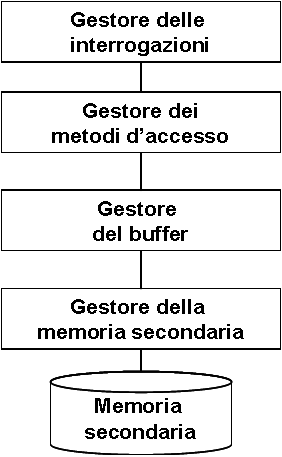
\includegraphics[width=5cm]{img/memsec.png}\\
  \caption{Schema dei moduli di gestione dei dati}\label{fig:schemod}
\end{figure}
\subsection{Memoria principale, memoria secondaria e gestione del buffer}
Le basi di dati hanno necessità di gestire dati in memoria secondaria per due motivazioni; la prima è che per quanto le dimensioni delle memorie centrali siano in costante aumento esse non riescono a soddisfare il fabbisogno della base di dati. In secondo luogo una delle caratteristiche delle basi di dati è la \emph{persistenza} e visto che le memorie centrali attualmente sono di tipo volatile non sono adatte a mantenere questa caratteristica.\\
Vediamo ora alcune caratteristiche della memoria secondaria, prima fra tutte come dice il nome stesso la memoria secondaria non può essere usata direttamente dai programmi, i dati per poter essere utilizzati devono prima essere caricati in memoria centrale. Sui dischi i dati sono memorizzati in \emph{blocchi} di dimensione (di solito) fissa di alcune decine di kilobyte. Le uniche operazioni possibili su un disco, come abbiamo già detto, sono le operazioni di lettura e scrittura di un intero blocco, questo significa che quando abbiamo bisogno anche di un solo bit dobbiamo caricare in memoria un intero blocco.\\
L'interazione tra memoria centrale e memoria secondaria è realizzata dai DBMS attraverso un apposita zona in memoria centrale detta \emph{buffer} gestita in modo condiviso dal DBMS per tutte le applicazioni. La gestione ottimale dei buffer è una questione essenziale in quanto permettono di evitare continui accessi alla memoria secondaria. Il buffer è organizzato in \emph{pagine} che hanno dimensione pari ad un numero intero di blocchi, per semplicità nel nostro caso imposteremo il numero di blocchi per pagina uguale a 1 e quindi non faremo distinzione tra i due termini.\\
Il \emph{gestore del buffer} si occupa del caricamento e dello scaricamento delle pagine dalla memoria centrale alla memoria di massa; possiamo pensare questo modulo come a un entità che riceve dai programmi richieste di lettura e scrittura su un blocco ed esegue le effettive letture e scritture sulla base di dati  secondo delle tempistiche che non coincidono con quelle di arrivo delle richieste; in particolare abbiamo che:
\begin{itemize}
  \item In caso di lettura, se la pagina è già presente nel buffer non è necessaria l'effettiva lettura fisica.
  \item In caso di scrittura il gestore può decidere di differire la scrittura fisica quando è possibile mantenere l'affidabilità del sistema.
\end{itemize}
Le politiche di gestione dei buffer assomigliano a quelle che il sistema operativo usa per la gestione della memoria centrale e obbediscono al principio di \emph{località dei dati} in base al quale i dati appena acceduti sono quelli con più alta probabilità che siano acceduti nell'immediato futuro.\\
La gestione del buffer è un po più complicata di così in quanto bisogna memorizzare informazioni sull'uso delle pagine che potremmo schematizzare nel seguente modo:
\begin{itemize}
  \item Un direttorio descrive il contenuto attuale del buffer indicano per ogni pagina quali sono il file fisico e il numero di blocchi ad essa corrispondenti.
  \item Per ogni pagina il gestore mantiene alcune variabili di stato fra cui un contatore dei programmi che usano quella pagina e un bit di stato per indicare se la pagina è stata modificata.
\end{itemize}
Un possibile insieme di operazioni che soddisfano queste caratteristiche sono le seguenti:
\begin{itemize}
  \item La primitiva \emph{fix} viene usata dalle transizioni per richiedere l'accesso ad una pagina e restituisce il riferimento alla pagina del buffer; l'esecuzione di tale operazione avviene nel seguente modo:
      \begin{enumerate}
        \item Si ricerca la pagina tra quelle già presenti in memoria, in caso positivo si ritorna l'indirizzo di memoria al richiedente
        \item Altrimenti si cerca una pagina libera del buffer cioè quelle con contatore pari a zero. Se il dirty bit è a uno allora essa viene scritta in memoria di massa.
        \item Se non esistono pagine libere possiamo avere due casi in base al comportamento del gestore del buffer, nel primo caso (politica \emph{steal}) viene sottratta una pagina ad un altra applicazione e la pagina viene scaricata in memoria di massa (operazione di \emph{flush}). Nel secondo caso (politica \emph{no steal}) la transizione viene sospesa fino alla liberazione di una pagina del buffer.
        \item In ogni caso quando viene effettuato un accesso alla pagina si incrementa il contatore relativo all'utilizzo di quella pagina.
      \end{enumerate}
  \item La primitiva \emph{setDirty} indica la modifica di una pagina e fa variare il bit relativo allo stato della pagina stessa
  \item La primitiva \emph{unfix} indica che il modulo chiamante ha terminato l'utilizzo della pagina e si ha come effetto il decremento del contatore.
  \item La primitiva \emph{force} forza il gestore del buffer a trascrivere in memoria la pagina in  modo sincrono
\end{itemize}
\subsection{Gestione delle tuple nelle pagine}
Sebbene ogni organizzazione fisica abbia una propria tecnica per la gestione delle pagine si sono alcuni aspetti comuni che possono essere interessanti da descrivere. In ciascuna pagina sono presenti due tipi di informazioni, l'informazione \emph{utile}, che coincide con i dati veri e propri e l'informazione di \emph{controllo} che consente di accedere alle informazioni.
\begin{figure}
  \centering
  % Requires \usepackage{graphicx}
  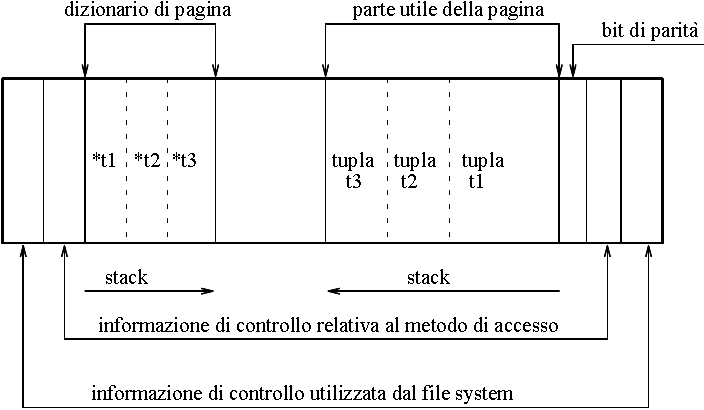
\includegraphics[width=15cm]{img/pagestr.png}\\
  \caption{Esempio di struttura di pagina}\label{fig:pagestr}
\end{figure}
Una possibile struttura di pagina è quella presentata in Fig. \ref{fig:pagestr} e qui descritta:
\begin{itemize}
  \item Ogni pagina, in quanto coincidente con un blocco ha una parte iniziale\emph{block header} e una finale \emph{block trailer} contente informazioni utilizzate dal filesystem.
  \item Ogni pagina in quanto contenete dati gestiti dal DBMS ha una parte iniziale (\emph{page header}) e una finale (\emph{page trailer}) contenenti informazioni di controllo specifiche alla struttura
  \item In molti casi ogni pagina ha un suo \emph{dizionario di pagina} che contiene un puntatore agli elementi della pagina e una \emph{parte utile} che contiene i dati. Dizionario di pagina e parte utile crescono solitamente come stack contrapposti lasciando così memoria libera in uno spazio contiguo.
  \item Infine ogni pagina contiene \emph{bit di parità} per verificare la correttezza dell'informazione.
\end{itemize}
In  molti casi non è possibile separare una tupla su più pagine così la massima dimensione della tupla è limitata a massimo spazio disponibile sulla pagine; in oltre molte volte le tuple hanno tutte quante la stessa dimensione, questo semplifica la struttura dei dizionari di pagina ma si corre il rischio di sprecare spazio nella pagina stessa.\\
Un parametro importante è il \emph{fattore di blocco} ovvero il numero di record contenuti in un blocco, che in prima approssimazione è pari al rapporto tra la dimensione del blocco e la dimensione media delle tuple.\\
Le primitive messe a disposizione dal gestore delle pagine sono:
\begin{description}
  \item[Inserimento e aggiornamento] che non comportano la riorganizzazione della pagina se esiste spazio sufficiente per la gestione della tupla. Se invece lo spazio non è contiguo le operazioni devono essere precedute da una riorganizzazione della pagina che però ha un costo limitato in quanto svolto in memoria centrale.
  \item[Cancellazione] essa è sempre possibile e viene fatta senza riorganizzare la pagina ma semplicemente marcando la tupla come "non valida".
  \item[Accesso a una tupla]  avviene tramite l'identificazione della valore della chiave o in base all'offset presente nel dizionario.
  \item[Accesso a un campo della tupla] identificato in base all'offset e alla lunghezza del campo stesso dopo aver identificato la tupla.
\end{description}
\subsection{Strutture primarie per l'organizzazione di file}
Le strutture con le quali vengono costruiti i file possono essere di tre tipi, \emph{sequenziali}, ad \emph{accesso calcolato} (o \emph{hash}) e ad \emph{albero}. Le strutture sequenziali sono caratterizzate da una struttura sostanzialmente consecutiva delle tuple in memoria di massa che deriva da una regola opportuna (istante di inserimento, valore di un campo).
Le strutture ad hash calcolano la posizione delle tuple in base ad un algoritmo. Le strutture ad albero, infine, sono utilizzate soprattutto come strutture secondarie.\\
\subsubsection{Strutture sequenziali}
Nelle strutture sequenziali un file è costituito da vari blocchi di memoria "logicamente" consecutivi e i le tuple vengono inserite nei blocchi rispettando una sequenza che può essere:
\begin{itemize}
  \item di tipo \emph{seriale (disordinata)} nel quale le tuple sono ordinate secondo l'ordine di immissione.
  \item un organizzazione ad \emph{array} nel quale le tuple sono disposte secondo il valore di un campo detto \emph{indice}.
  \item una organizzazione \emph{sequenziale ordinata} nel quale l'organizzazione dipende dal valore assunto in ciascuna tupla da un campo del file.
\end{itemize}
\paragraph{Struttura seriale (disordinata)}
In questo tipo di struttura gli inserimenti avvengono alla fine del file in modo sequenziale e sono perciò molto efficienti, basta gestire un puntatore all'ultima tupla inserita. I problemi si presentano nel caso di cancellazione e modifica di una tupla in quanto la cancellazione spreca memoria, mentre la modifica, nel caso di aumento di memoria, comporta una ristrutturazione dell'intero file.
Questa struttura è anche chiamata \emph{entry-sequence} per sottolineare il metodo di inserimento o \emph{heap} per specificare che i dati sono "ammucchiati" senza nessun ordine.\\
Questa tipo di struttura è molto efficiente per quanto riguarda letture e scritture ma molto meno efficiente quando si tratta della ricerca di un singolo dato all'interno del file. Per ovviare a questo problema, nelle basi di dati relazionali queste tipi di strutture (le più utilizzate visto la semplicità di implementazione e gestione) vengono affiancate da strutture secondarie.
\paragraph{Struttura sequenziale ad array} Le strutture ad array sono implementabili solo nel caso in cui le tuple siano di dimensioni fissa, in questo caso allora al file vengono associati \emph{n} blocchi contigui con $m$ spazzi per il salvataggio delle tuple dando luogo ad un array di dimensione $n\times m$ ciascuna tupla viene dotata di un indice $i$ e viene posta nella posizione $i$-esima dell'array.\\
Le primitive garantite da questa organizzazione sono quelle di inserimento, lettura e cancellazione; gli inserimenti iniziali avvengono semplicemente incrementando l'indice mentre le cancellazione lasciano delle posizioni libere, i successivi inserimenti vanno a riempire queste posizioni libere o avvengono in fondo al file.\\
Le strutture ad array non vengono quasi mai utilizzate nei DBMS in quanto, nella maggior parte dei casi, le tuple non rispettano le condizioni iniziali di questa struttura.
\paragraph{Struttura sequenziale ordinata} L'organizzazione sequenziale ordinata assegna a ciascuna tupla una posizione in base al valore di un campo detto \emph{chiave}. Sono così avvantaggiate le operazioni che richiedono un accesso ordinato alle tuple di una tabella in base alla chiave, ed inoltre è possibile effettuare ricerche dicotomiche.\\
Questo tipo di struttura non è più utilizzato in tempi recenti in quanto vi è un problema fondamentale nell'inserimento di nuove tuple che richiede un eccessivo overhead per la gestione di queste strutture. Infatti l'inserimento di una nuova tupla implica sempre o quasi sempre il riordino delle altre tuple. Alcuni meccanismi che possono migliorare questo problema sono:
\begin{itemize}
  \item Prevedere a priori un certo numero di posizioni libere all'atto del caricamento iniziale in modo da permettere un successivo riordino "locale".
  \item Inserire nuovi blocchi a seguito di saturazioni ma questa porta a rinunciare alla contiguità dei blocchi.
  \item integrare il file sequenziale ordinato con \emph{file di overflow} dedicato a gestire le tuple che eccedono lo spazio disponibile, i diversi file di overflow sono collegati tra loro da una \emph{catena di overflow} che parte da un blocco del file ordinato.
\end{itemize}
\subsubsection{Strutture ad accesso calcolato}
Una struttura ad accesso calcolato garantisce, come la struttura sequenziale ordinata, un accesso \emph{associativo} ai dati, ovvero il posizionamento fisico dei dati dipende da un valore assunto da un campo chiave; a differenza però della struttura sequenziale, quella ad hash, non necessita che i dati siano fisicamente sequenziali. La struttura viene realizzata allocando al file un numero $B$ di blocchi (sovradimensionando il file e non riempiendo completamente i blocchi si ottiene un funzionamento migliore).\\
L'idea è quella di estendere le caratteristiche di accesso degli array anche nel caso in cui questi non siano applicabili. Gli array si prestano a realizzare una struttura per organizzare dati che abbiano un campo chiave con valori consecutivi. Mentre nel caso nel caso il numero degli elementi è molto più piccolo dei valori possibili per il campo chiave la tecnica sequenziale degrada velocemente. Volendo però usare una struttura simili a quella degli array si può pensare di trasformare il campo chiave in un indice di un array; per fare ciò si utilizza un algoritmo e la funzione di trasformazione è detta \emph{funzione di hash}. Il problema principale di questo tipo di struttura è il fatto che il campo chiave è molto più grande dei possibili valori dell'indice e perciò la funzione di hash non può essere iniettiva ed è quindi possibile che si verifichino collisioni, ovvero chiavi con valori diversi ma che portano allo stesso valore di indice. Anche se una buona funzione di hash rende bassa la probabilità di collisione l'unico modo per abbassare effettivamente le collisioni è aumentare lo spazio disponibile.\\
Ora, traendo vantaggio dalla proprietà della memoria secondaria che l'operazione di accesso ad un blocco ha costo unitario e che un blocco può contenere diversi record, e dato che si tende a non riempire completamente un blocco ma si tende a mantenere un certo \emph{fattore di riempimento} per allocare la giusta quantità di blocchi per memorizzare un certo numero di record con una funzione di hash si può usare la formula:
$$B=\left\lceil\frac{T}{f \times F}\right\rceil$$
Dove $T$ è il numero di tuple previsto per il file $f$ è il fattore di riempimento e $F$ il fattore di blocco (numero di record per blocco).
In caso di collisione i record vengono semplicemente allocati nel blocco fino ad esaurimento dello spazio e quando questo è esaurito viene allocato un ulteriore blocco e i nuovi record vengono allocati in esso dando così luogo a \emph{catene di overflow}.\\
La struttura hash è ideale quando si vuole effettuare un \emph{accesso puntuale} ad un record tramite la sua chiave ma le prestazioni degradano pesantemente in caso di accesso ad un certo intervallo di valori della chiave in quanto la funzione di hash tende a disperdere i dati. Mentre non si ha alcun vantaggio quando si vuole accedere ad un qualsiasi altro campo della tupla.
\subsection{Strutture ad albero}
In questo paragrafo studieremo le strutture ad albero denominate \emph{indici}, esse sono strutture che favoriscono l'accesso in base al valore di uno o più campi sia nel caso di accessi puntuali sia nel caso di accessi ad intervalli. Le strutture ad albero possono essere utilizzate sia per la costruzione di strutture primarie, ovvero contenete i dati, sia strutture secondarie che favoriscono solamente gli accessi ai dati.\\
\subsubsection{Indici primari e secondari}
Daro un file $f$ con un campo chiave $k$ un \emph{indice secondario} è un altro file in cui ogni record è composto da due campi uno contenete un valore della chiave $k$ e l'altro contente l'indirizzo fisico del record in $f$. L'indice secondario è ordinato in base alla chiave perciò consente una rapida ricerca in base a quel valore. Nel caso in cui, invece, l'indice contiene al suo interno anche i dati esso è detto \emph{indice primario} perché non garantisce l'accesso solo in base alla chiave ma contiene anche i dati stessi. Un file può avere un solo indice primario e più indici secondari.\\
Della struttura ad albero possiamo analizzare alcune caratteristiche:
\begin{itemize}
  \item Nel primo caso gli indirizzi fisici si riferiscono solo ai blocchi di memoria nel quale il dato è contenuto, oppure possono contenere gli offset all'interno del blocco. Le due soluzioni se pur diverse sono paragonabili in termini di prestazioni. I puntatori ai blocchi sono più compatti mentre i puntatori ai record permettono di rendere più efficenti alcune interrogazioni.
  \item Un indice primario, grazie al suo ordinamento, può essere realizzato puntando ad un solo record per ciascun blocco; in questo caso si dice che l'indice è \emph{sparso}. In caso di indice secondario, invece, esso deve contenere per forza tutti i riferimenti della chiave visto che valori consecutivi della chiave possono trovarsi in blocchi differenti. in questo caso si parla di indice \emph{denso}.
\end{itemize}
Per quanto riguarda le prestazioni in ogni caso la caratteristica degli indici è quella di permettere ricerche efficienti sia nel caso di range che di singolo record, inoltre, gli indici sono solitamente più piccoli dei file a cui fanno riferimento e quindi le ricerche possono essere più efficienti.
\subsubsection{Strutture ad albero dinamiche}
Le strutture ad albero dinamiche del tipo \emph{B-tree} o \emph{B+-tree} sono le più usate nei DBMS relazionali per la realizzazione degli indici. Ogni albero ha un nodo radice, vari nodi intermedi e vari nodi foglia, ogni nodo coincide cono una pagina o blocco a livello di file system e di gestore del buffer. I legami tra i nodi vengono stabiliti da puntatori che collegano fra loro le pagine, ogni nodo ha un numero di discendenti abbastanza grande che dipende dall'ampiezza della pagina. Si costruiscono così alberi con un numero \emph{limitato di livelli} nei quali la maggioranza dei nodi è costituita da nodi foglia.\\
Un altro requisito fondamentale per un  buon funzionamento di queste strutture dati è che gli alberi siano \emph{bilanciati} ovvero che la lunghezza del cammino che collega il nodo radice con qualsiasi nodo foglia sia pressochè identica e pari alla profondità dell'albero.\\
\paragraph{Contenuto dei nodi e tecnica di ricerca}
\begin{figure}
  \centering
  % Requires \usepackage{graphicx}
  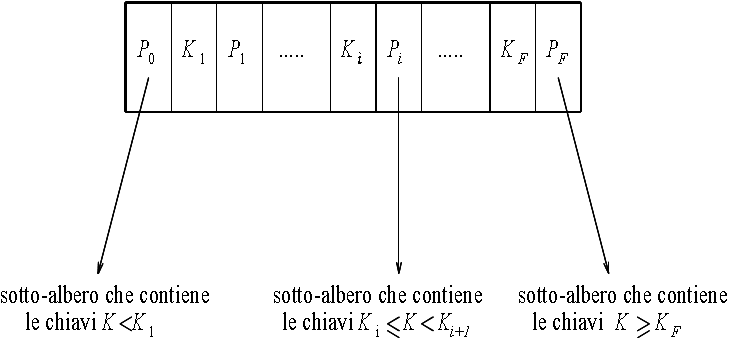
\includegraphics[width=14cm]{img/nodo.png}\\
  \caption{Esempio di nodo intermedio}\label{fig:nodo}
\end{figure}
La struttura tipica di un nodo è mostrata in figura \ref{fig:nodo}, esso presenta una sequenza di $F$ valori ordinati di chiave. Ogni chiave $K_i$ con $1\leq i \leq F$ è seguita da un puntatore $P_i$. $K_1$ è preceduta da un puntatore $P_0$. Ciascun puntatore punta ad un sotto-albero così definito:
\begin{itemize}
  \item Il puntatore $P_0$ punta al sotto-albero che contiene quei record con chiave \emph{minore} di $K_1$.
  \item Il puntatore $P_F$ indirizza al sotto-albero che contiene i record con chiavi \emph{maggiori o uguali} di $K_F$
  \item Gli altri puntatori puntano ciascuno ad un sotto-albero che contiene i  valori delle chiavi compresi tra i due valori $K_i$ e $K_{i+1}$
\end{itemize}
In sintesi ciascun nodo contiene $F$ valori di chiave e $F+1$ puntatori ad altri nodi, dove $F+1$ è detto \emph{fan-out} dell'albero; mentre $F$ dipende dall'ampiezza della pagina e dalla dimensione dei valori di chiave nella parte "utile" della pagina, si sceglie per $F$ il massimo valore possibile in modo da ridurre i livelli dell'albero.\\
La primitiva di ricerca nelle strutture ad albero è molto semplice in quanto consente un accesso associativo alla tupla che contiene la chiave $V$. Il meccanismo di ricerca consiste nel seguire i puntatori partendo dalla radice e considerando le seguenti regole:
\begin{itemize}
  \item se $V < K_1$ si segue il puntatore $P_0$
  \item se $V > K_F$ si segue il puntatore $P_F$
  \item altrimenti si segue il puntatore $P_j$ tale per cui $K_j \leq V <K_{j+1}$
\end{itemize}
e la ricerca prosegue fino ai nodi voglia dell'albero che possono essere organizzati nei due seguenti modi:
\begin{itemize}
  \item Nel primo caso i odi contengono l'intera tupla e la struttura dati che si ottiene è detta \emph{index-sequential} e permette la realizzazione di un file ordinato con un associato indice primario. La posizione della tupla è vincolata dal campo chiave. Cancellazione e inserimento non risultano però complicate in quanto la posizione viene stabilita dinamicamente.
  \item Nel secondo caso ciascun nodo foglia contiene puntatori ai blocchi della base di dati. La struttura che si ottiene in questo caso è detta \emph{indiretta}. La posizione delle tuple può essere qualsiasi e in questo caso si potrebbe indirizzarle con qualsiasi altro indice primario.
\end{itemize}
Inserimenti e cancellazioni non provocano grossi problemi nel caso in cui nel nodo vi sia spazio. Nel caso di inserimento in un nodo in cui non vi sia spazio a sufficienza si effettua un'operazione di \emph{split} che divide l'informazione già presente nella foglia più quella nuova in due foglie dal peso equilibrato. Questa operazione può provocare lo split anche ai nodi superiori fino a risalire la radice.\\
una cancellazione invece può essere sempre fatta in loco ma può portare a due problematiche:
\begin{itemize}
  \item Quando in un indice sparso la cancellazione coinvolge uno dei valori chiave è opportuno recuperare il successivo valore chiave e inserirlo al posto del valore cancellato.
  \item Quando una cancellazione lascia due foglie semivuote tanto che l'informazione in esse contenuta possa essere contenuta in una sola allora si deve svolgere un operazione di \emph{merge} che non è altro che il duale dell'operazione di split
\end{itemize}
\begin{figure}
  \centering
  % Requires \usepackage{graphicx}
  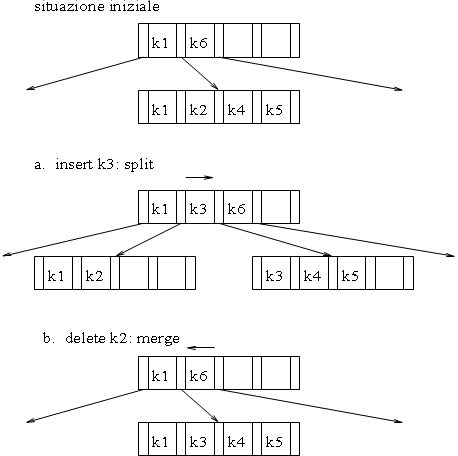
\includegraphics[width=10cm]{img/split.png}\\
  \caption{Esempio di operazioni di split (a) e di merge (b)}\label{fig:split}
\end{figure}
La modifica del valore di un campo chiave viene trattata come una cancellazione del suo valore iniziale seguito da un inserimento del valore finale.
\paragraph{Alberi B e B+}
Esistono due versioni della struttura ad albero, gli alberi di tipo B e quelli di tipo B+. La distinzione è abbastanza semplice, infatti, negli alberi di tipo B+ i nodi foglia sono collegati da una catena che li connette in base all'ordine della chiave; questo fa si che le interrogazioni il cui predicato definisce un intervallo di valori siano svolte in modo efficiente. In questo caso è sufficiente trovare il primo valore dell'intervallo per poi scandire il resto dei risultati in sequenza (Fig. \ref{fig:B+tree}).\\
Nel caso degli alberi di tipo B è possibile effettuare una ottimizzazione aggiungendo ad ogni chiave un puntatore che punta direttamente al record mentre l'altro puntatore punta al sottoalbero per continuare la ricerca (Fig. \ref{fig:Btree})
\begin{figure}
  \centering
  % Requires \usepackage{graphicx}
  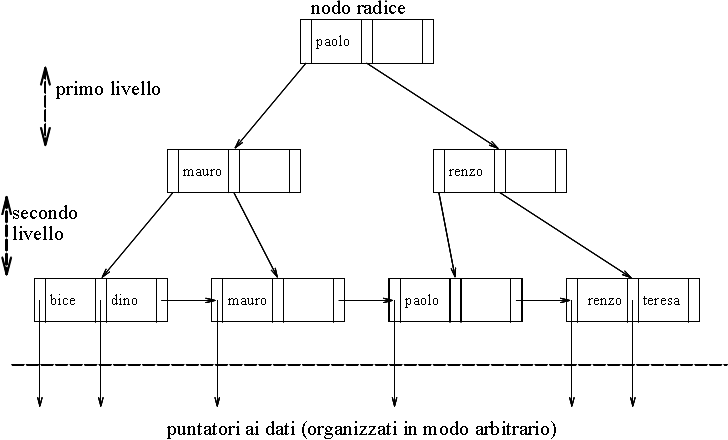
\includegraphics[width=12cm]{img/bptree.png}\\
  \caption{Albero di tipo B+}\label{fig:B+tree}
\end{figure}
\begin{figure}
  \centering
  % Requires \usepackage{graphicx}
  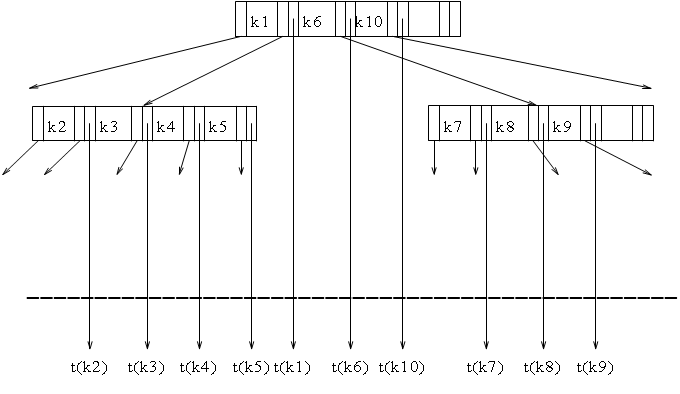
\includegraphics[width=12cm]{img/btree.png}\\
  \caption{Albero di tipo B}\label{fig:Btree}
\end{figure}
\subsection{Strutture fisiche e indici nei DBMS relazionali}
I DBMS attualmente in commercio differiscono in modo sostanziale per i dettagli sulle strutture fisiche che mettono a disposizioni, ma possiamo trovare alcuni principi generali sui quali la maggior parte dei DBMS si basa.\\
in particolare, tutti i sistemi prevedono una struttura di base di tipo seriale disordinata su cui è possibile definire inidici secondari. Quasi tutti i sistemi creano un indice per la chiave primaria in quanto questo rende più semplice verificare il rispetto del vincolo.
Molti sistemi prevedono la possibilità di memorizzare in modo contiguo le tuple di una tabella con gli stessi valori su un certo campo, questa tecnica prende il nome di \emph{cluster}. In molti casi si tratta di un vero e proprio ordinamento fisico, in altri è associata ad una funzione di hash o ad un indice.\\
Tutti i sistemi permettono la realizzazione di indici e praticamente tutti prevedono la realizzazione tramite B+-tree, mentre alcuni sistemi prevedono anche altri tipi di indice. Un altro tipo di indice è il cossiddetto \emph{indice hash} ovvero una struttura secondaria realizzata tramite l'accesso calcolato.
\subsection{Gestore delle interrogazioni: esecuzione e ottimizzazione}
Il gestore delle interrogazioni è un modulo cruciale dell'architettura di un DBMS in quanto responsabile dell'esecuzione \emph{efficiente} dell'operazioni che sono specificate a livello molto alto. Esso riceevve in ingresso un interrogazione SQL essa viene analizzata per indivuduare eventuali errori sintattici o semantici; in questa fase il sistema accede al \emph{dizionario dei dati} per leggere le informazioni in esso contenute ed effettuare i controlli. Una volta accettata l'interrogazione viene tradotta in una forma interna di tipo algebrico. A questo punto inizia la fase di ottimizzazione:
\begin{itemize}
  \item Viene svolta in primo luogo un'ottimizzazione di tipo algebrico che consiste nell'effettuare tutte le trasformazioni algebriche necessarie. Questa ottimizzazione avviene indipendentemente dal modello dei costi assunto dal sistema.
  \item In secondo luogo, viene svolta una ottimizzazione che dipende sia dalla tipologia dei metodi di accesso ai dati sia dal modello dei costi.
  \item Infine si genera il codice che utilizza i metodi di accesso ai datti, ovvero, si ottengono i \emph{programmi di accesso} in formato "interno" che richiedono l'uso delle strutture dati fornite dal sistema.
\end{itemize}
Al contrario di altri moduli l'ottimizzazione delle interrogazioni agisce a tempo di compilazione. Nel caso in cui l'interrogazione venga compilata una sola volta ed eseguita molteplici (\emph{complie and store}) il codice viene memorizzato nella base di dati. Nel caso in cui l'interrogazione venga compilata e immediatamente eseguita (\emph{compile and go}) il codice non viene memorizzato.
\subsubsection{Profili delle relazioni}
Ciascun DBMS contiene informazioni quantitative relative alle caratteristiche delle tabelle dette \emph{profili delle relazioni} che vengono memorizzate nel dizionario dei dati, alcuni di questi profili sono:
\begin{itemize}
  \item La \emph{cardinalità}, $CARD(T)$, ovvero il numero di tuple di ciascuna tabella T.
  \item La \emph{dimensione} in byte, $SIZE(T)$, di ciascuna tupla di T.
  \item La \emph{dimensione} in byte, $SIZE (A_j,T)$ di ciascun attributo di T.
  \item Il \emph{numero di valori distinti}, $VAL(A_j,T)$ di ciascun attributo $A_j$ di T.
  \item Il \emph{valore minimo}, $MIN(A_j,T)$, e quello \emph{massimo}, $MAX(A_j,T)$ di ciascun attributo di T.
\end{itemize}
I profili vengono calcolati in base ai dati effettivamente memorizzati nella tabella tramite l'ausilio di opportune primitive di sistema, ma è compito dell'amministratore richiamare periodicamente \texttt{update statics} per aggiornare questi profili.
\subsubsection{Rappresentazione interna delle query}
La rappresentazione che viene data dall'pttimizzatore ad una interrogazione tiene conto della struttura fisica utilizzata per implementare le tabelle, nonché degli indici disponibili su di esse. Perciò la prima trasformazione consiste nel rappresentare l'interrogazione con una struttura ad albero nella quale i nodi foglia corrispondono a strutture fisiche (tabelle, indici, file) e i nodi intermedi sono aoperazioni di accesso ai dati che sono supportati dalle strutture fisiche.
\paragraph{Operazione di scansione}
Un'operazione di \emph{scansione} (\emph{scan}) esegue diverse operazioni sia di ti tipo algebrico che non algebrico:
\begin{itemize}
  \item proiezione su di una lista di attributi
  \item selezione di un predicato
  \item inserimento cancellazioni e modifiche delle tuple quando vi si fa accesso durante la scansione
\end{itemize}
Le primitive che interessano questa operazione sono:
\begin{center}
  \texttt{open, next, read, modify, insert, delete,close}
\end{center}
\paragraph{Ordinamenti}
La necessità di operazioni di ordinamento emerge sia ai fini delle applicazioni (eseguite per lo più in memoria centrale tramite meccanismi ad hoc) sia per una corretta realizzazione di proiezioni con eliminazione dei duplicati (spesso eeseguita su grandi file tramite la composizione di sort su parti dei file e merge finale).
\paragraph{Accesso diretto}
 Si usa il termine \emph{accesso diretto} quando è possibile accedere ad uno o più record senza dover necessariamente esaminare il file in modo sequenziale, ma tramite indici; questo si ha nel caso in cui i predicati siano semplici ($A_i = V$) o intervalli ($V_1<A_i<V_2$), in questi casi si dice che il predicato dell'interrogazione è \emph{valutabile} tramite l'indice.\\
 Nel caso l'interrogazioni presenti un solo predicato valutabile la convenienza è quella di effettuare la ricerca tramite indice. Nel caso sia una \emph{congiunzione} di predicati valutabili allora si sceglie il più selettivo per l'accesso diretto mentre il secondo viene valutato in memoria centrale tramite \emph{scan}. Nel caso in cui l'interrogazione presenti una \emph{disgunzione} dei predicati basta che uno solo non sia valutabile che si rende necessaria una ricerca tramite scan.
 \paragraph{Metodo di join}
\begin{figure}
  \centering
  % Requires \usepackage{graphicx}
  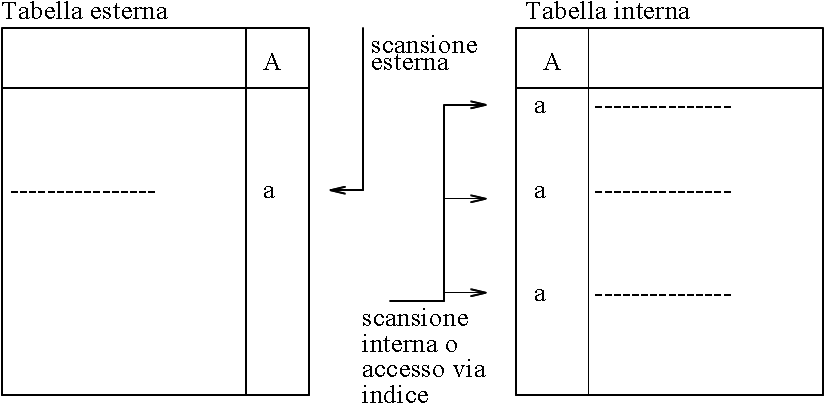
\includegraphics[width=13cm]{img/nested.png}\\
  \caption{Nested-loop join}\label{fig:nested}
\end{figure}
\begin{figure}
  \centering
  % Requires \usepackage{graphicx}
  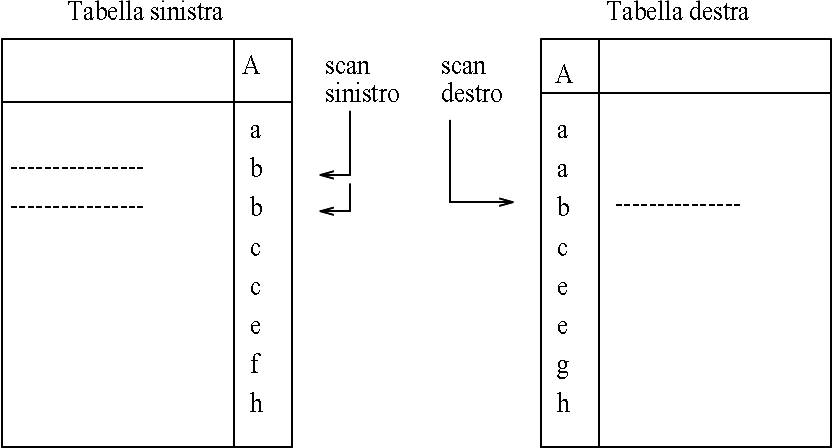
\includegraphics[width=13cm]{img/merge.png}\\
  \caption{Merge-scan join}\label{fig:merge}
\end{figure}
\begin{figure}
  \centering
  % Requires \usepackage{graphicx}
  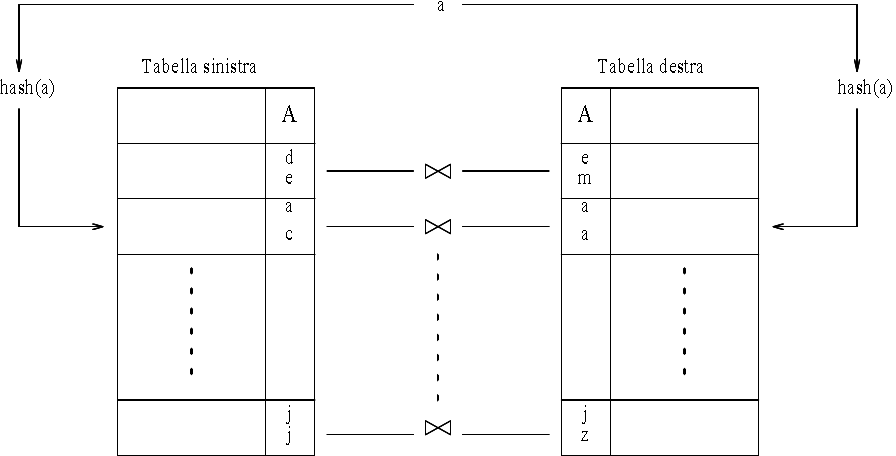
\includegraphics[width=13cm]{img/hashed.png}\\
  \caption{Hashed join}\label{fig:hashed}
\end{figure}
 Il join è l'operazione più costosa per un DBMS in quanto vi è il rischio di una esplosione del numero di tuple del risultato; un join su campi che non siano chiave per nessuno dei due operandi può avere un numero di tuple uguale al prodotto della cardinalità degli operandi stessi.\\
 Vediamo ora tre tipologie di realizzazione del join
 \begin{description}
   \item[Nested loop] Nel nested loop (Fig. \ref{fig:nested}) una tabella viene definita come \emph{esterna} mentre l'altra come \emph{interna}. Si esegue una scansione sulla tabella esterna e per ogni tupla individuata si preleva il valore dell'attributo e si ricerca tale valore nella tabella interna tramite una scansione o l'utilizzo di un indice \emph{ad hoc} sull'attributo cercato. Questa tecnica non ha un costo fisso ma dipende dalla disponibilità di spazio nel buffer e della tecnica di ricerca nella tabella interna
   \item[Merge scan] Questa tecnica (Fig. \ref{fig:merge}) richiede di esaminare le tabelle secondo l'ordine dell'attributo di join ed è quidi efficente quando le tabelle sono già ordinate o esistono degli indici adeguati. Viene eseguita mediante scansioni parallele sulle due tabelle come nei classici algoritmi di \emph{merge}; quando gli attributi coincidono allora vengono generate ordinatamente tuple del risultato
   \item[Hash-based] Questo metodo rapprfesentato in Fig. \ref{fig:hashed} viene eseguito in due passi: nel primo passo una funzione di hash $h$ applicata sugli attributi di join viene utilizzata per creare una copia ordinata di ciascuna delle due tabelle. La funzione $h$ fa corrispondere i valori di dominio di tali attributi a $B$ partizioni su ciascuna tabella. Le tuple con gli stessi valori dell'attributo di join saranno poste nelle stesse partizioni. Sarà così poi sufficiente effettuare B semplici join tra le partizioni a pari indice.
 \end{description}
 Il costo di queste tecniche non può essere valutato in astratto a priori ma dipende dalle scelte che precedono o seguono il join.
 \subsubsection{Ottimizzazione basata sui costi}
 L'ultimo passaggio che porta a definire il piano di accesso è assai difficile sul piano computazzionale in quanto sono presenti varie dimensioni di ottimizzazione.
 \begin{itemize}
   \item Occorre scegliere quali operazioni di accesso ai dati svolgere, in particolare, nel primo accesso ai dati occorre talvolta scegliere tra una scansione e un accesso tramite indici. 
   \item Occorre scegliere l'ordine delle operazioni da compiere
   \item Quando è possibile occorre scegliere fra le varie alternative per la realizzazione di una operazione (esempio il metodo di join)
   \item Quando l'interrogazione o il metodo di realizzazione richiedono un ordinamento bisogna stabilire a quale livello della strategia svolgere tale operazione.
 \end{itemize}
 Di fronte a questa complessità gli ottimizzatori dispongono di formule di costo approssimate. Essi costrruiscono un \emph{albero delle alternative} (Fig. \ref{fig:alterna}) in cui ogni nodo corrisponde a fissare una particolare opzione fra quelle elencare sopra. Ogni nodo foglia dell'albero corrisponde ad una specifica \emph{alternativa di esecuzione} della interrogazione descritta dalle scelte che si trovano percorrendo l'albero dalla radice fino al nodo foglia. Il problema è così riformulato nella ricerca del nodo foglia con costo minore.\\
\begin{figure}
  \centering
  % Requires \usepackage{graphicx}
  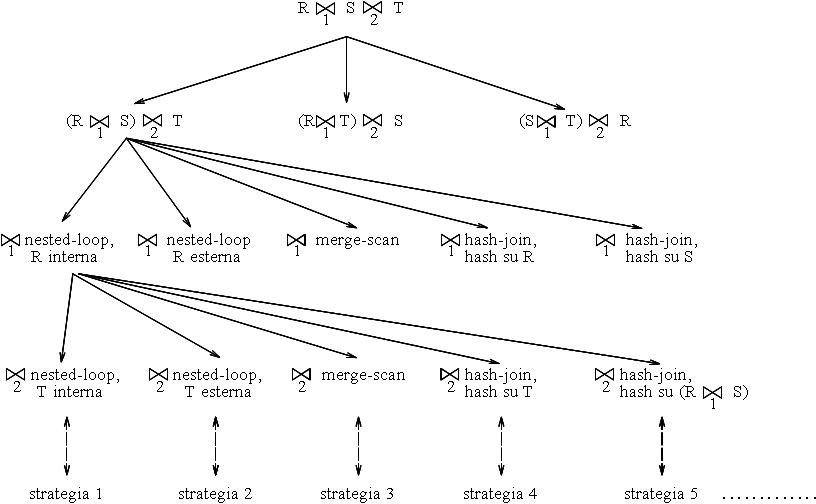
\includegraphics[width=12cm]{img/alterna.png}\\
  \caption{Albero delle alternative per un join su tre tabelle}\label{fig:alterna}
\end{figure}
 Il problema viene tipicamente risolto tramite formule di costo che associano a ciascuna operazione intermedia un costo in termini di operazioni di I/O e di istruzioni necessarie a valutarne il risultato.
 $$C_{total} = C_{I/O} \times n_{I/O} + C_{cpu} \times n_{cpu}$$
 Dove $C_{I/O},\ C_{cpu}$ sono parametri noti e $n_{I/O},\ n_{cpu}$ indicano il numero di operazioni di ingresso uscita e di istruzioni necessarie per valutare il risultato dell'interrogazione.\\
 Talvolta la strategia ottimale richiede la realizzazione di strutture ad hoc per svolgere le operazioni, in questo caso sono da considerare anche i costi di costruzione di tali strutture. 

\end{document}
